\documentclass[journal]{IEEEtran}

\usepackage{amsmath,amssymb}
\usepackage{array}
\usepackage{booktabs}
\usepackage{cite}
\usepackage{graphicx}
\usepackage{multirow}
\usepackage[hidelinks]{hyperref}
\usepackage{xcolor}

\title{An Audited Evaluation of Event-Aware Retrieval for 24-hour PM2.5 Forecasting}

\author{Sabbir Hossain%
\thanks{S. Hossain is with the Department of Computer Science and Engineering,
American International University-Bangladesh, Dhaka, Bangladesh.}}

\begin{document}

\maketitle

\begin{abstract}
While retrieval augmentation can provide a convenient method to provide forecasting models with historical analogues, the idea can be misleading when the memory is limited, when the comparison baseline is weak, and when individual contextual channels are not tested independently. This study performs an audit of the Event-TimeRAF retrieval framework, which consists of a Source-Audited Context Builder, Leakage-Safe Event-Context Retriever and a Drift-Aware Forecast and Evidence Head. EPA AirData PM2.5, NOAA Global Hourly weather, calendar variables and hash-verified NOAA Storm Events data are aligned for Los Angeles County from 2019 to 2024. The lookback for evaluation is 168 hours, the horizon is 24 hours, the number of test origins is 7,199, the number of knowledge-base strides is four, the event-weight controls are used, and the retrieval placebos are applied, with overlap-aware paired inference. The weather-calendar XGBoost baseline model has the best performance as indicated by the MSE of 26.185, MAE of 3.125, RMSE of 5.117, and $R^2$ of 0.379. The full Event-TimeRAF model achieves MSE 26.734, and its difference from the context baseline is unresolved. Frozen Chronos-Bolt obtains MSE 28.941, retrieval fusion obtains 28.733, but a climatology fusion control obtains 27.450 and significantly outperforms the retrieval fusion. A denser six-hour memory reduces retrieval-only MSE to 34.616, but the corresponding feature model remains behind the context baseline. An increase in the event weight results in 91.4\% of the test top-k sets being changed, but also has a negative effect on retrieval error, suggesting that the tested event representation does not provide forecast value. Since Storm Events does not have publication timestamps, event-conditioned findings are retrospective sensitivity results.
\end{abstract}

\begin{IEEEkeywords}
Forecasting, PM2.5, retrieval-augmented forecasting, time-series foundation models, event context, distribution-shift diagnostics, forecast traceability.
\end{IEEEkeywords}

\section{Introduction}

Fine particulate matter (PM2.5) is one of the key urban air-quality risks as it is related to respiratory and cardiovascular health impacts \cite{who2021airquality}. Public-health alerts, exposure-reduction, transport planning and environmental operations can all benefit from accurate short-range PM2.5 forecasts. However, in Los Angeles County, PM2.5 dynamics are not as easily modeled using pollutant history. Concentrations may vary according to wind speeds, boundary-layer conditions, rain, seasonal activity, holidays, wildfire smoke, and unusual storms and/or high wind conditions. These factors render the problem of forecasting as being temporal and contextual.

Recent time-series foundation models (TSFMs) have been designed to enhance the generalization of forecasting, with the goal of pre-training on extensive time-series corpora and adapting the forecasting capability to other domains. Some examples of models are TimesFM, Moirai, MOMENT, Chronos and Tiny Time Mixers \cite{das2024timesfm,woo2024moirai,goswami2024moment,ansari2024chronos,ekambaram2024ttm}. Concurrently, retrieval-augmented generation (RAG) has demonstrated how nonparametric memory can be leveraged to enable access to the relevant external knowledge at inference time for foundation models \cite{lewis2020rag,karpukhin2020dpr}. TimeRAF merges the two concepts for zero-shot time-series forecasting: retrieving sequences from a curated knowledge base that are relevant to the target sequence and passing them as input to a ``frozen'' TSFM using Channel Prompting \cite{zhang2025timeraf}.

The domain for air-quality forecasting introduces a retrieval problem which has not only a numerical time-series aspect but also a domain-specific aspect. A historical PM2.5 window is a window that is similar to the current window, but under other weather or event conditions. On the other hand, if the window is moderately similar in terms of numbers, but shares high wind, rain, holiday, smoke or stagnation context, then this window may provide more information. This encourages a retrieval system where source records, weather, calendar data, and distribution-shift indicators are all considered part of the forecasting evidence, and not just metadata unrelated to the forecast.

This work assesses Event-TimeRAF, a retrieval-augmented framework for PM2.5 forecasting under distribution shift, which is event-aware. The approach is an adaptation of the retrieval principle of TimeRAF in an official-source environment, and does not pretend to be reproducing the learned retriever or Channel Prompting of TimeRAF. The Event-TimeRAF consists of 3 named components: the Source-Audited Context Builder (SACB), Leakage-Safe Event-Context Retriever (LSER), and Drift-Aware Forecast and Evidence Head (DFEH). These components aim to answer three questions: how to map official environmental records to a retrieval-friendly context; how to choose historical candidates without temporal leakage; and when retrieval is beneficial in addition to a strong supervised weather-calendar baseline.

The contributions are the following:
\begin{itemize}
    \item \textit{Source-Audited Context Builder:} a reproducible mechanism that aligns EPA PM2.5, NOAA weather, calendar and hash-verified NOAA Storm Events records while ensuring source identity, coverage checks, and the assumed event availability.
    \item \textit{Leakage-Safe Event-Context Retriever:} a historical analogue mechanism that enforces a query--candidate embargo and is evaluated using memory density, neighbour count, event weight, and event-stratified controls.
    \item \textit{Drift-Aware Forecast and Evidence Head:} a controlled evaluation layer comparing direct XGBoost, frozen Chronos-Bolt, retrieval fusion and non-retrieval fusion placebos while preserving machine-readable shift and provenance evidence.
\end{itemize}

The assessment is made on a conservative basis. It only allows claims of a single manifest-backed run, presents 2,000-resample paired block intervals, presents overlap-aware Diebold--Mariano tests and does not presume that event association is the same as causation. The negative results differentiate a working retrieval pipeline that can be audited from evidence that retrieval improves forecasting.
\section{Literature Review and Related Work}

\subsection{Statistical, Machine-Learning, and Deep Forecasters}
Different forecasting methods trade off inductive bias, data requirements and computational requirements. The autoregressive and seasonal models continue to serve as informative baseline models, whose failure modes can be examined. Tree ensembles like XGBoost and LightGBM can be used to further expand this space to nonlinear lag, rolling, weather, and calendar interactions without a sequence encoder \cite{chen2016xgboost,ke2017lightgbm}. RNNs such as LSTMs and GRUs, however, learn a stateful temporal representation \cite{hochreiter1997lstm,cho2014gru}. Large benchmark archives are also available, such as the Monash Forecasting Repository, which enables the possibility of being able to compare and reproduce results across different domains of time series \cite{godahewa2021monash}. For transformer families, they stress long-term dependencies, such as Informer that lowers attention cost, Autoformer and FEDformer which decompose temporal variation, Crossformer and iTransformer which model the cross-variable structure, and TimesNet which reorganizes temporal variation into 2D patterns \cite{zhou2021informer,wu2021autoformer,zhou2022fedformer,zhang2023crossformer,liu2024itransformer,wu2023timesnet}. The benefits of these gains do not suggest that more complicated architecture is (always) required. Simple decomposition or patch-based inductive biases like DLinear and PatchTST can still be very competitive \cite{zeng2023dlinear,nie2023patchtst} while TimeMixer adopts explicit multiscale decomposition and mixing \cite{wang2024timemixer}. Event-TimeRAF therefore retains seasonal and boosted tree baselines instead of assuming that a deep backbone is the default winner.

\subsection{Time-Series Foundation Models}
Time-series foundation models (TSFMs) aim to transfer knowledge between datasets instead of learning fresh representations for each time-series. TimesFM is a decoder-only forecasting design; Moirai is a universal forecasting Transformer; MOMENT supports multiple time-series tasks; Chronos is a value-to-token forecasting model; and Tiny Time Mixers focuses on compact zero- and few-shot transfer \cite{das2024timesfm,woo2024moirai,goswami2024moment,ansari2024chronos,ekambaram2024ttm}. Generative pretraining, long-context scaling, cross-domain unification or language-model reprogramming are the focus of Timer, Timer-XL, UniTime, and Time-LLM \cite{liu2024timer,liu2025timerxl,liu2024unitime,jin2024timellm}. Frozen pretrained models have also been tested as generic time-series computation engines \cite{zhou2023onefitsall}. In total, these studies encourage zero-shot evaluation, while also demonstrating the importance of input representation and domain shift to transfer performance. The present study thus compares frozen Chronos-Bolt with locally supervised models on the same forecast origins without assuming foundation-model superiority.

\subsection{Retrieval-Augmented Forecasting}
Retrieval augmentation is the dissociation of parametric knowledge from an external memory. The retrieve-then-condition paradigm was pioneered in NLP by RAG and Dense Passage Retrieval \cite{lewis2020rag,karpukhin2020dpr}. Diffusion forecasting and assisted generation workflows are used to study retrieval in time series \cite{liu2024ratd,ang2024tsgassist}. The most similar methodology is provided by TimeRAF \cite{zhang2025timeraf}, which builds a time-series knowledge base and trains an MLP dual-encoder retriever; then it selects the top-k candidates and introduces embeddings of the candidates into the frozen TSFM using Channel Prompting. Its ablations examine retrieval quality, integration, number of candidates, knowledge-base composition, and backbone choice.

Event-TimeRAF is inspired by the external memory principle and addresses a different experimental question. It uses transparent random, cosine and event-context retrieval controls instead of a learned dual encoder, and feature- or forecast-level fusion instead of internal Channel Prompting. This difference does not allow the current implementation to be called a copy of TimeRAF, but rather an audited environmental adaptation that tests whether contextual historical analogues improve a local PM2.5 task.

\subsection{Air-Quality Forecasting and Official Context}
PM2.5 prediction is usually combined with the histories of pollutants, and with temperature, humidity, wind, precipitation and pressure. Recent reviews suggest a trend towards using attention-based, hybrid, and spatiotemporal models in place of single-station recurrent models \cite{zhou2024pm25review,zhang2023sparsepm25}. For instance, AirFormer can isolate the deterministic spatiotemporal modelling from the stochastic uncertainty estimation at a national level \cite{liang2023airformer}. These multi-station designs include a spatial dependence, while the present study deals with an aggregate at county level and with the origin of contextual evidence. EPA AirData provides regulated PM2.5 measurements, NOAA Integrated Surface Database provides hourly meteorological data, and NOAA Storm Events provides structured hazard data \cite{epaairdata2026,noaaisd2026,noaastormevents2026}. Smoke evidence could be added from NOAA Hazard Mapping System products, but were not included in the reported run \cite{noaahms2026}.

\subsection{Distribution Shift and Forecast Explanations}
Means, variances and relationships between inputs and future values can change with temporal nonstationarity. Adaptive normalization methods estimate statistics at local temporal scales \cite{liu2023san}; Event-TimeRAF instead defines interpretable shift indicators to audit the regimes without claiming that shift has been eliminated. The range of explanation methods is also varied. SHAP assigns predictions to model inputs \cite{lundberg2017shap} and information-theoretic saliency helps with counterfactual inspection of probabilistic forecasts \cite{raman2023forecast}. The explanation layer that was implemented is narrower, as it only contains signed XGBoost effects, retrieved cases, event identifiers, drift components and a diagnostic uncertainty scale. These records provide the basis for traceability without establishing causal effects from events or weather.
\section{Critical Gaps and Limitations of Previous Studies}

Prior work leaves three interrelated gaps in event-sensitive urban air-quality forecasting. First, the provenance, coverage and availability assumptions of local context records may not be carried over to temporal forecasters and numerical retrieval systems. A numerically similar PM2.5 window may be brought about by a different weather or event regime and a retrospective event label may be misinterpreted as a piece of information available at forecast time. The SACB fills this gap by putting the official data under explicit audits of source, coverage and availability.

Secondly, historical retrieval may suffer from look-ahead bias if there is an overlap of the query context with a candidate input or target. Similarity alone does not prevent a near-duplicate future from entering the retrieved evidence. The LSER fills this void by means of a temporal embargo and a training-history restriction, followed by separately auditable PM2.5, weather, calendar and event similarity terms.

Third, gains from retrieval are often not tested against a strong local context model which captures the useful signal, whether they hold up under distribution shift, or whether an explanation can be traced to stored evidence. The DFEH tackles this shortcoming by comparing direct XGBoost and frozen Chronos-Bolt paths on common origins, exposing shift indicators, and maintaining machine-readable feature, retrieval, event and uncertainty evidence. It is not an explanation of causation, but a component which enables comparisons and auditability.

These mappings mark the boundaries of the new material in the study. Event-TimeRAF does not use a learned dual-encoder retriever or internal Channel Prompting, and the current experiment is limited to a single county, thus not directly demonstrating geographic generalization.

\section{Core Contributions}

The proposed framework provides three mechanisms, which map one-to-one to the above gaps:
\begin{itemize}
    \item \textit{Source-Audited Context Builder (SACB):} creates an aligned 85-dimensional context with official PM2.5, meteorological, calendar and event records and metadata on the sources and availability.
    \item \textit{Leakage-Safe Event-Context Retriever (LSER):} retrieves training-history analogues after enforcing a candidate-target embargo and exposes the contribution of each similarity channel and the retrieved trajectory evidence.
    \item \textit{Drift-Aware Forecast and Evidence Head (DFEH):} provides one chronological evaluation contract for direct horizon models, frozen-TSFM forecast fusion, drift-state analysis and traceable explanation records.
\end{itemize}

The empirical contribution is made deliberately tentative: while the weather-calendar context results in the most noticeable reduction in error, denser retrieval results in an improvement only in the retrieval-only path, and the event channel tested does not result in an improvement in forecast accuracy.
\section{Problem Formulation}

Let $x_t$ be the measurement of PM2.5 concentration at time $t$. The historical air-quality lookback window for forecast time $t$ is:
\begin{equation}
    X_t = [x_{t-L+1}, x_{t-L+2}, \ldots, x_t],
    \label{eq:lookback}
\end{equation}
where $L$ is the length of the lookback window. Let $W_t$ be weather covariates that correspond to the lookback window, $C_t$ be calendar features and $E_t$ be event context available at the forecast origin under the recorded source assumption. The target associated with the input in Equation~(\ref{eq:lookback}) is defined in Equation~(\ref{eq:target}).
\begin{equation}
    Y_{t+1:t+H} = [x_{t+1}, x_{t+2}, \ldots, x_{t+H}],
    \label{eq:target}
\end{equation}
where $H$ is the forecasting horizon. Equation~(\ref{eq:target}) gives the 24-step vector at every valid forecast origin.

The objective of forecasting is to learn a function
\begin{equation}
    \hat{Y}_{t+1:t+H} =
    F_{\theta}(X_t, W_t, C_t, E_t, R^{ts}_t, R^{ev}_t, D_t),
    \label{eq:forecast}
\end{equation}
where $R^{\mathrm{ts}}_t$ is retrieved time-series knowledge, $R^{\mathrm{ev}}_t$ is retrieved event knowledge and $D_t$ contains concept-drift indicators. The target setting that has been implemented is $L=168$ hours and $H=24$ hours. The complete information interface is given in Equation~(\ref{eq:forecast}); the modules which build these arguments are detailed in the following section.

This evaluation is based on a split of time:
\begin{equation}
    \mathcal{T}_{train} < \mathcal{T}_{val} < \mathcal{T}_{test},
    \label{eq:chronological_split}
\end{equation}
The first 70\% of observations are used for training, the next 15\% for validation and the last 15\% for testing. The ordering in Equation~(\ref{eq:chronological_split}) is used for feature fitting, retrieval eligibility, model selection and evaluation.

The essential notation is summarized in Table~\ref{tab:symbols}.

\begin{table}[!t]
\centering
\caption{Main Symbols Used in the Proposed Formulation}
\label{tab:symbols}
\begin{tabular}{ll}
\toprule
Symbol & Meaning \\
\midrule
$L$ & Lookback window length \\
$H$ & Forecast horizon \\
$X_t$ & Historical PM2.5 sequence at time $t$ \\
$W_t$ & Weather covariates \\
$C_t$ & Calendar/context features \\
$E_t$ & Event context available at the forecast origin \\
$R^{ts}_t$ & Retrieved time-series knowledge \\
$R^{ev}_t$ & Retrieved event knowledge \\
$D_t$ & Drift indicators \\
$q_t$ & SACB context vector in $\mathbb{R}^{85}$ \\
$G_t$ & LSER top-$k$ retrieved set \\
$\rho(G_t)$ & Retrieval summary in $\mathbb{R}^{51}$ \\
$\mathcal{O}_t$ & Machine-readable DFEH evidence record \\
$\hat{Y}_{t+1:t+H}$ & Predicted future PM2.5 values \\
\bottomrule
\end{tabular}
\end{table}
\section{Methodology}

Event-TimeRAF consists of three main parts. The Source-Audited Context Builder (SACB) transforms heterogeneous official records into a chronological context of hours and adds provenance and availability metadata. The Leakage-Safe Event-Context Retriever (LSER) builds an embargoed historical memory, which it uses to retrieve analogues based on PM2.5, weather, calendar and event similarity. The Drift-Aware Forecast and Evidence Head (DFEH) reveals the feature-level and forecast-level prediction paths, indications of shifts and a machine-readable explanation record. These components operate on one-dimensional time-series and tabular inputs; they do not imply an image operator, learned attention block or TimeRAF Channel Prompting.

\subsection{Framework Overview and Forward Pass}

The entire dataflow is summarized in Figure~\ref{fig:architecture}. The first step involves auditing the EPA PM2.5, NOAA weather, calendar, and NOAA Storm Events records and putting them into a query context as well as input--target windows. The LSER filters, ranks and returns aligned candidate futures and retrieval statistics from the training-history knowledge base. The DFEH then feeds those statistics to 24 direct XGBoost regressors, evaluates a separate frozen Chronos-Bolt fusion path, calculates the drift evidence and writes the forecast and supporting record.

\begin{figure*}[!t]
\centering
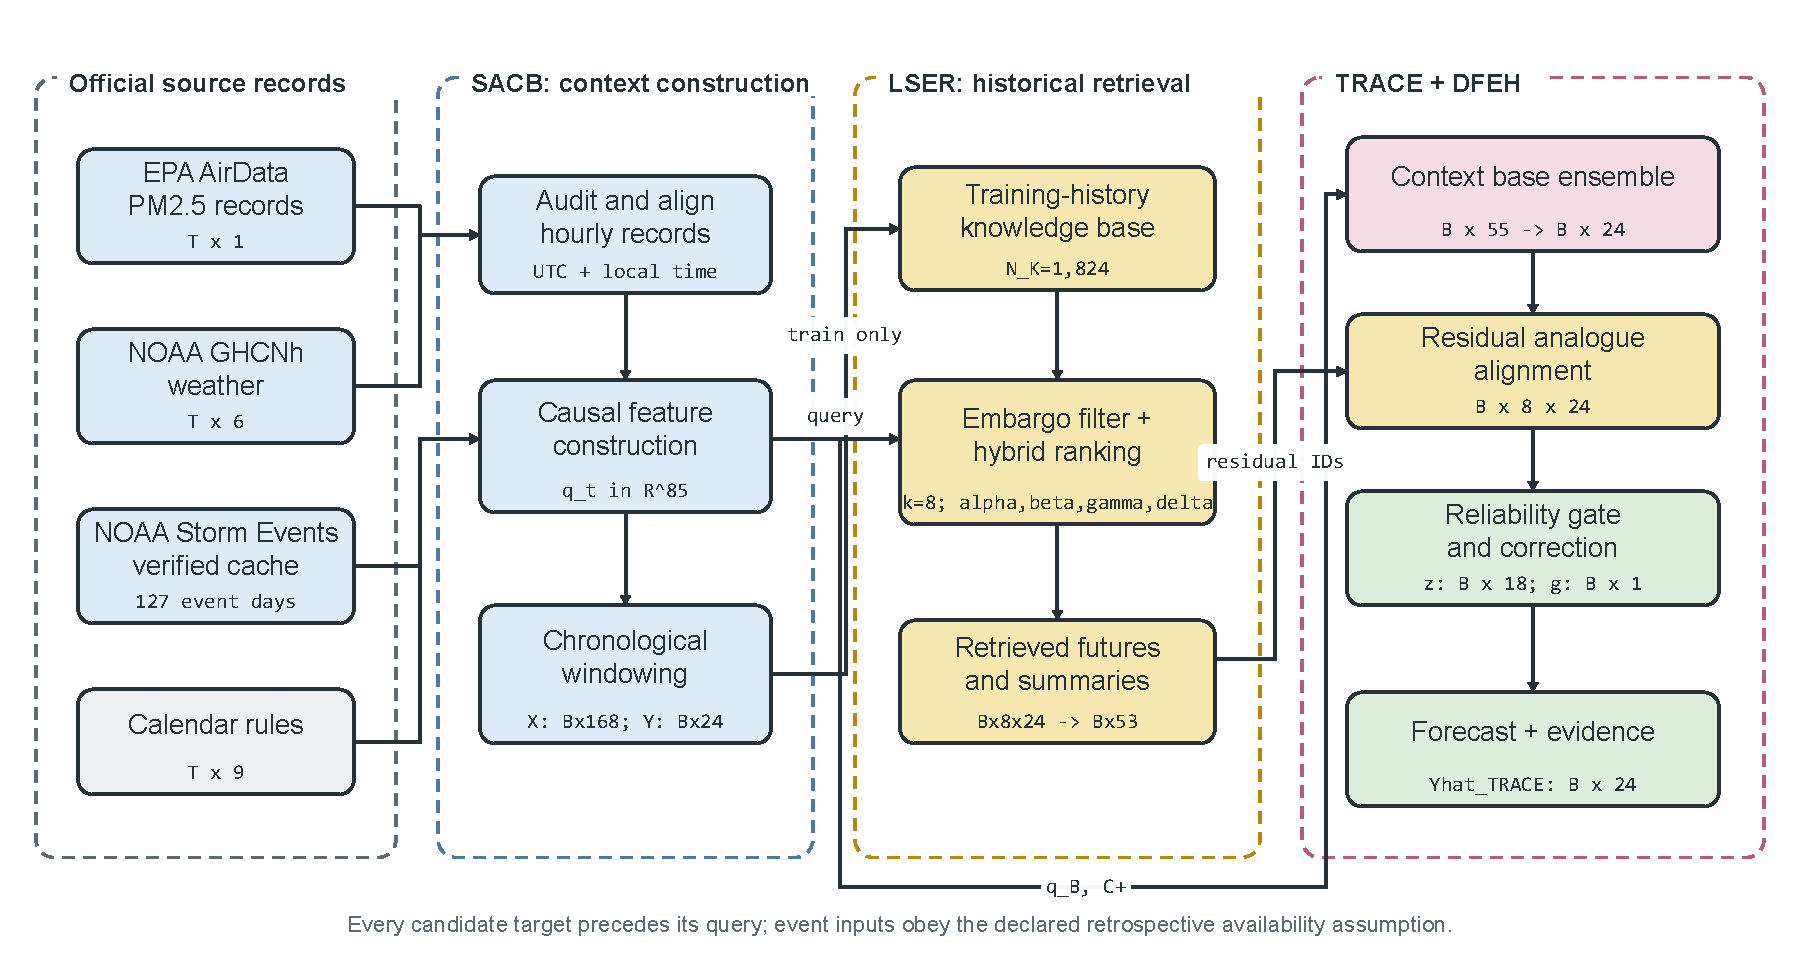
\includegraphics[width=\textwidth]{figures/event_timeraf_pipeline_overview.pdf}
\caption{Proposed Event-TimeRAF pipeline. Official records pass through the
Source-Audited Context Builder (SACB), training-history candidates are selected
by the Leakage-Safe Event-Context Retriever (LSER), and the Drift-Aware
Forecast and Evidence Head (DFEH) produces 24-hour forecasts and traceable
evidence. Tensor annotations show the reported configuration.}
\label{fig:architecture}
\end{figure*}

Event-TimeRAF maps the aligned context into a forecast for each forecast origin $t$,
\begin{equation}
    \hat{Y}_{t+1:t+H} =
    F_{\theta}\bigl(\phi(X_t,W_t,C_t,E_t), G_t, D_t\bigr),
    \label{eq:event_timeraf_mapping}
\end{equation}
The tabular feature construction $\phi(\cdot)$, retrieved historical evidence $G_t$ and drift evidence $D_t$ are used. The availability requirement is that all components of $G_t$ and $D_t$ have to be available by the time the forecast is made. The forward pass below is the expansion of Equation~(\ref{eq:event_timeraf_mapping}) at the tensor level.

The batch of B origins can be expanded out in tensor notation as follows for the forward pass that is actually implemented:
\begin{equation}
\begin{aligned}
Q &= \operatorname{SACB}(X,W,C,E) &&\in \mathbb{R}^{B\times 85},\\
G &= \operatorname{LSER}(Q,\mathcal{K}) &&\in \mathbb{R}^{B\times 8\times 24},\\
U_h &= [Q\,\|\,\rho(G)\,\|\,d\,\|\,C^{+}_{h}]
&&\in \mathbb{R}^{B\times 151},\\
\hat{Y}^{X} &= [f_1(U_1),\ldots,f_{24}(U_{24})]
&&\in \mathbb{R}^{B\times 24},\\
(\hat{Y},\mathcal{O}) &= \operatorname{DFEH}
(\hat{Y}^{X},\hat{Y}^{C},\hat{Y}^{R},d,G)
&&\in \mathbb{R}^{B\times 24}\times\mathcal{E},
\end{aligned}
\label{eq:forward_pass}
\end{equation}
where Q is the origin context in 85 dimensions, $\rho(G)\in\mathbb{R}^{B\times 51}$ is the retrieved trajectory, spread, two similarity summaries and candidate count, $d\in\mathbb{R}^{B\times 6}$ is the five drift components and their mean score, and $C^{+}_{h}\in\mathbb{R}^{B\times 9}$ is the known calendar vector for horizon $h$. The symbol $\mathcal{E}$ denotes the schema $\mathcal{O}$ of the evidence record. Equation~(\ref{eq:forward_pass}) describes both forecasting paths without presenting the XGBoost path as part of the frozen foundation model.

\subsection{Source-Audited Context Builder}

The SACB's driving force is to maintain data provenance and temporal availability prior to model fitting. Source-specific checks come before the construction of features as illustrated in Figure~\ref{fig:context_builder}. EPA monitor data are combined into a county hourly median, NOAA weather data are synchronized from the selected surface station, event data archives are hash-checked against a manifest, and calendar data are calculated from the local timestamp. The resulting context is then windowed and split chronologically, with no interpolation of target values.

\begin{figure*}[!t]
\centering
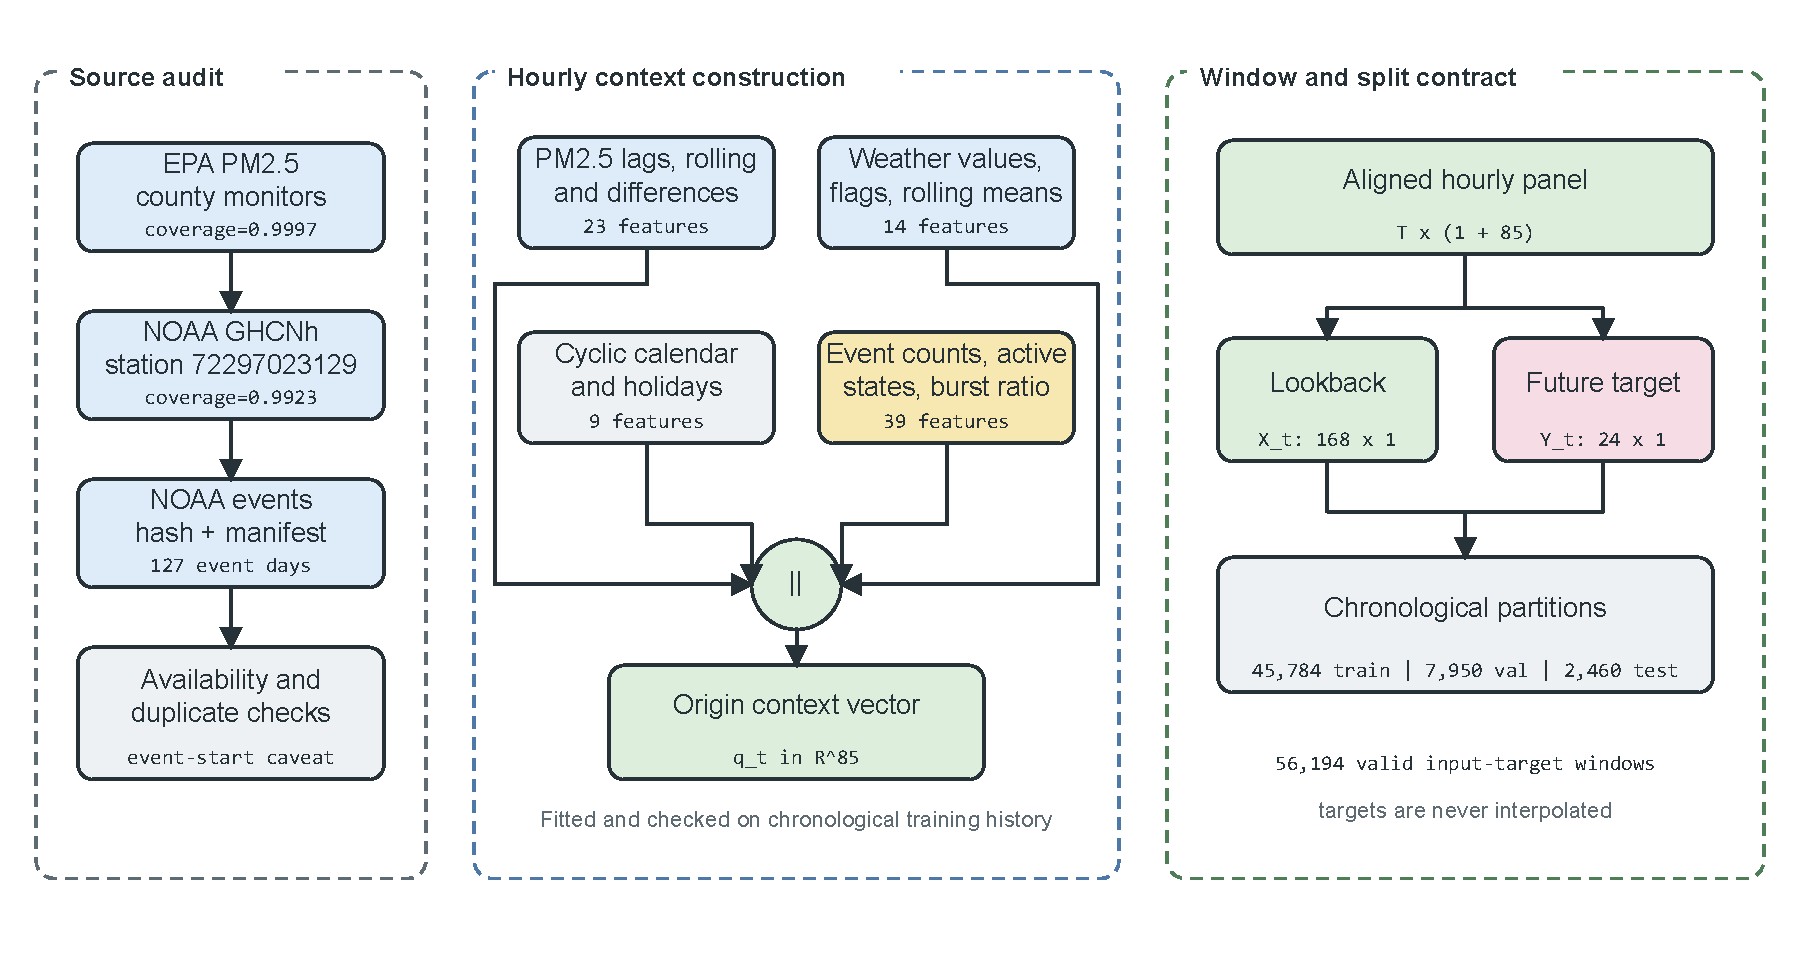
\includegraphics[width=\textwidth]{figures/source_audited_context_builder.pdf}
\caption{Source-Audited Context Builder. Source checks feed four feature groups
that form an 85-dimensional origin vector. The aligned panel is converted into
168-hour inputs and 24-hour targets before the chronological split.}
\label{fig:context_builder}
\end{figure*}

\subsubsection{Dataset Construction}
The data are hourly measurements of PM2.5 concentrations from US EPA AirData/AQS parameter 88101, in Los Angeles County \cite{epaairdata2026}. If a single monitoring site meets the coverage criterion, then the data audit selects this site using the coverage and continuity criteria. The target is the hourly county median measured by official Los Angeles County AQS monitors because no single monitor met this criterion. Timestamps are converted to \texttt{America/Los\_Angeles} with daylight-saving time explicitly handled. No targets are ever interpolated and only observations from before the gap are allowed to be used for a short gap in the input. The weather covariates are obtained from the closest available NOAA Integrated Surface Database (ISD) station \cite{noaaisd2026}. Calendar features include weekend status, weekday, month and cyclic hour terms, US federal holidays and California holidays.

The groups of features are flattened as
\begin{equation}
q_t=[p_t\,\|\,w_t\,\|\,c_t\,\|\,e_t]
\in\mathbb{R}^{23+14+9+39}=\mathbb{R}^{85},
\label{eq:context_vector}
\end{equation}
where $p_t$, $w_t$, $c_t$ and $e_t$ are the feature vectors for PM2.5, weather, calendar and events, respectively. Fixed lags, rolling moments and extrema, differences, current value and a fill flag are included in the PM2.5 group. The weather group consists of six measured variables, a precipitation-missing flag, derived condition flags and 24-hour rolling means. The event group includes one-hour and active counts, 24-, 72- and 168-hour counts, category-specific 72-hour counts and an event-burst ratio. Thus, Equation~(\ref{eq:context_vector}) specifies the feature ordering and the 85-dimensional SACB output used by the downstream modules.

Normalization statistics are only fit on the train split. The same normalization is applied to query and candidate windows, and the principle of TimeRAF is to have the same convention for the preprocessing of the sequences to be retrieved as well as those that are input. The reported run contains 48,332 valid windows with $X\in\mathbb{R}^{48332\times168}$ and $Y\in\mathbb{R}^{48332\times24}$.

\subsection{Leakage-Safe Event-Context Retriever}

The LSER distinguishes between temporal eligibility and relevance. The embargo is first displayed in Figure~\ref{fig:retrieval_timeline}: a candidate is considered only if its complete target precedes the beginning of the query lookback. The eligible candidates are then compared according to four separately stored similarity channels. The chosen futures are scaled to match the query scale and summarized for the forecasting head. This ordering prevents a high similarity score from overriding the temporal constraint.

\begin{figure*}[!t]
\centering
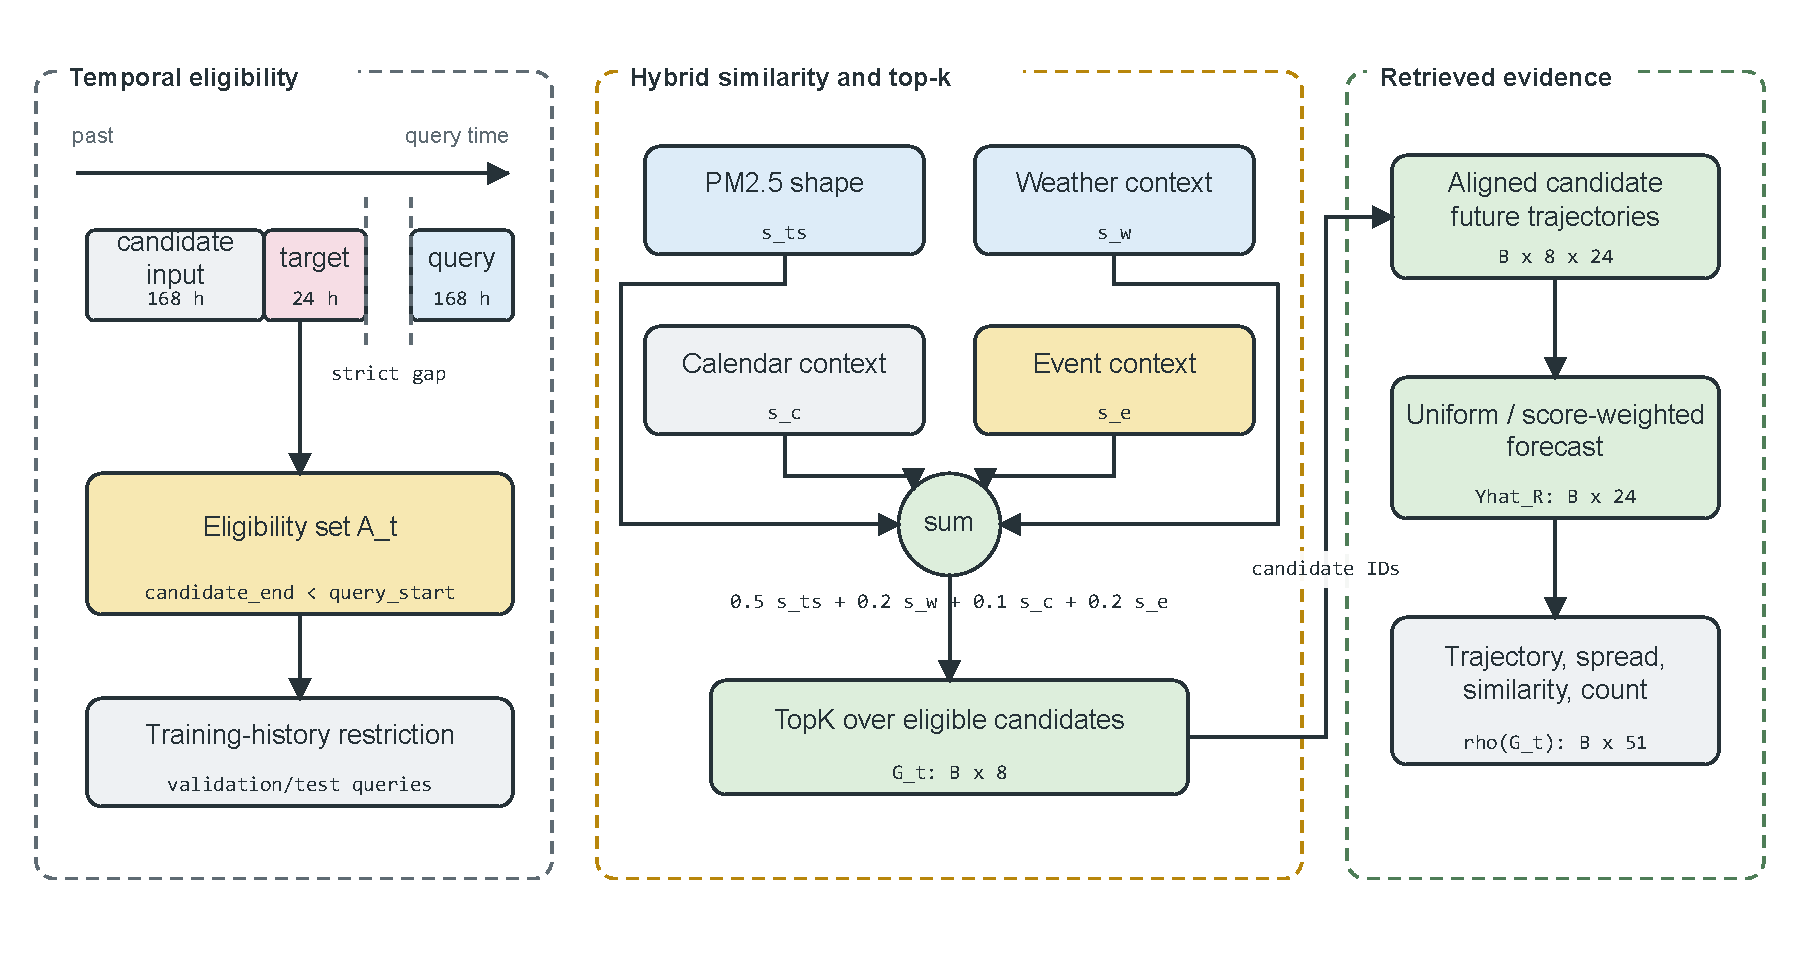
\includegraphics[width=\textwidth]{figures/leakage_safe_event_context_retriever.pdf}
\caption{Leakage-Safe Event-Context Retriever. A strict candidate-target
embargo and training-history restriction are applied before hybrid ranking.
The top eight candidates provide aligned future trajectories and a
51-dimensional retrieval summary.}
\label{fig:retrieval_timeline}
\end{figure*}

\subsubsection{Time-Series Knowledge Base}
Historical PM2.5 windows are placed in the time-series knowledge base. A window identifier, start time, end time, input and future values, weather summary, calendar summary, normalized window vector, split and a normalization identifier are stored in each record. The main setting uses a 24-hour origin stride and has 1,521 training-history candidates. Candidate windows may overlap each other; the query--candidate embargo is enforced by Equation~(\ref{eq:eligible_set}). Sensitivity experiments use 192-, 24-, 6-, and 1-hour strides, producing 191, 1,521, 5,644, and 34,020 candidates, respectively.

Formally, a knowledge base is
\begin{equation}
    \mathcal{K} = \{(u_i, X_i, Y_i, m_i, c_i, e_i)\}_{i=1}^{N},
    \label{eq:knowledge_base}
\end{equation}
where $u_i$ is the candidate origin, $X_i$ and $Y_i$ are the candidate lookback and future windows, $m_i$ is a weather summary, $c_i$ is a calendar summary and $e_i$ is the event-context summary available at $u_i$. The set of temporally eligible sets for query origin $t$ is
\begin{equation}
    \mathcal{A}_t =
    \{i: u_i + H < t-L+1,\; i \in \mathcal{T}_{train}\},
    \label{eq:eligible_set}
\end{equation}
For validation and test queries, the inequality in Equation~(\ref{eq:eligible_set}) is strict and guarantees that a candidate's target period ends before the query input period starts. The training-history condition in Equation~(\ref{eq:eligible_set}) also applies to final validation and test retrieval. The stored candidate schema is defined in Equation~(\ref{eq:knowledge_base}), and the subset admissible at query time is defined in Equation~(\ref{eq:eligible_set}).

Given a query window $X_t$, the time-series retriever returns
\begin{equation}
    R^{ts}_t = \{r^{ts}_{t,1}, r^{ts}_{t,2}, \ldots, r^{ts}_{t,k}\},
    \label{eq:retrieved_set}
\end{equation}
where $k$ is the number of retrieved candidates. The default is $k=8$, with sensitivity analysis for $k\in\{1,4,8,16\}$. Equation~(\ref{eq:retrieved_set}) is the result of the returned records prior to summarization of their future trajectories.

\subsubsection{Event Knowledge Base}
The event knowledge base comprises source-preserving information about events in Los Angeles County. NOAA Storm Events is the required structured source, while NOAA Hazard Mapping System fire and smoke records remain an unmeasured optional extension \cite{noaastormevents2026,noaahms2026}. The stored fields are event identifier, start, end, information-availability assumption, location, category, source, source URL, title and summary. The reported records show wildfire, high wind, heavy rain, flood and other weather categories; feature slots for absent configured categories remain zero.

The model inputs include hourly event counts, 24-, 72-, and 168-hour rolling event counts, 72-hour event counts by category, active event counts and an event-burst ratio. Recent source identifiers are retained as explanation evidence. Target-horizon overlap is not given as input to the models and can only be used as a post-hoc subset label. Because NOAA Storm Events has no machine-readable publication time, the implementation records event start as a retrospective availability assumption. Publication or issue times are needed for strict operational experiments.

\subsubsection{Hybrid Ranking and Future Alignment}
Query and candidate PM2.5 windows are standardized by their own means and standard deviations and normalized to unit length. Weather and calendar groups are standardized using candidate statistics, and their cosine similarities are mapped to [0, 1]. Event similarity is clipped to [0, 1] with explicit zero-vector handling. The hybrid retrieval score is the combination of the time-series similarity, weather relevance, calendar relevance and event relevance:
\begin{equation}
    s(q, i) =
    \alpha s_{ts}(q,i) +
    \beta s_{w}(q,i) +
    \gamma s_{c}(q,i) +
    \delta s_{e}(q,i),
    \label{eq:hybrid_score}
\end{equation}
The time-series similarity $s_{ts}$, the weather similarity $s_w$, the calendar similarity $s_c$, and the event relevance $s_e$ are used. The implemented weights are $\alpha=0.5$, $\beta=0.2$, $\gamma=0.1$, and $\delta=0.2$. In equation~(\ref{eq:hybrid_score}), each relevance channel is kept explicit to inspect the contribution of each channel without a learned latent scoring function.

The retrieved set is chosen as
\begin{equation}
    G_t = \operatorname{TopK}_{i \in \mathcal{A}_t}\; s(t,i).
    \label{eq:topk}
\end{equation}
Equation~(\ref{eq:topk}) is evaluated only after applying $\mathcal{A}_t$. Candidate futures are restored to the query scale as
\begin{equation}
\widetilde{Y}_{t,i}=\mu_t+\sigma_t
\left(\frac{Y_i-\mu_i}{\max(\sigma_i,\epsilon)}\right),
\qquad i\in G_t,
\label{eq:future_alignment}
\end{equation}
Here $(\mu_t,\sigma_t)$ and $(\mu_i,\sigma_i)$ are the query and candidate lookback statistics, and $\epsilon=10^{-6}$ avoids division by zero. The retrieval-only forecasts average $\widetilde{Y}_{t,i}$ uniformly or by non-negative normalized scores. The feature-level path retains the mean trajectory, horizon-wise spread, mean and maximum time-series similarity, and candidate count, resulting in $\rho(G_t)\in\mathbb{R}^{51}$. The affine transformation in Equation~(\ref{eq:future_alignment}) maintains the shape of the candidate trajectory and restores the local scale of the query.

\subsection{Drift-Aware Forecast and Evidence Head}

DFEH is the common output layer for the two verified forecasting paths, as well as the evidence output. The direct path, as depicted in Figure~\ref{fig:explanation_flow}, concatenates context, retrieval, drift and future-calendar features for 24 individually trained XGBoost regressors. A second path evaluates frozen Chronos-Bolt and combines its forecast with the retrieved forecast at a validation-selected weight. Drift scores and flags are kept as diagnostic inputs and evidence fields, not for selecting between forecasters.

\begin{figure*}[!t]
\centering
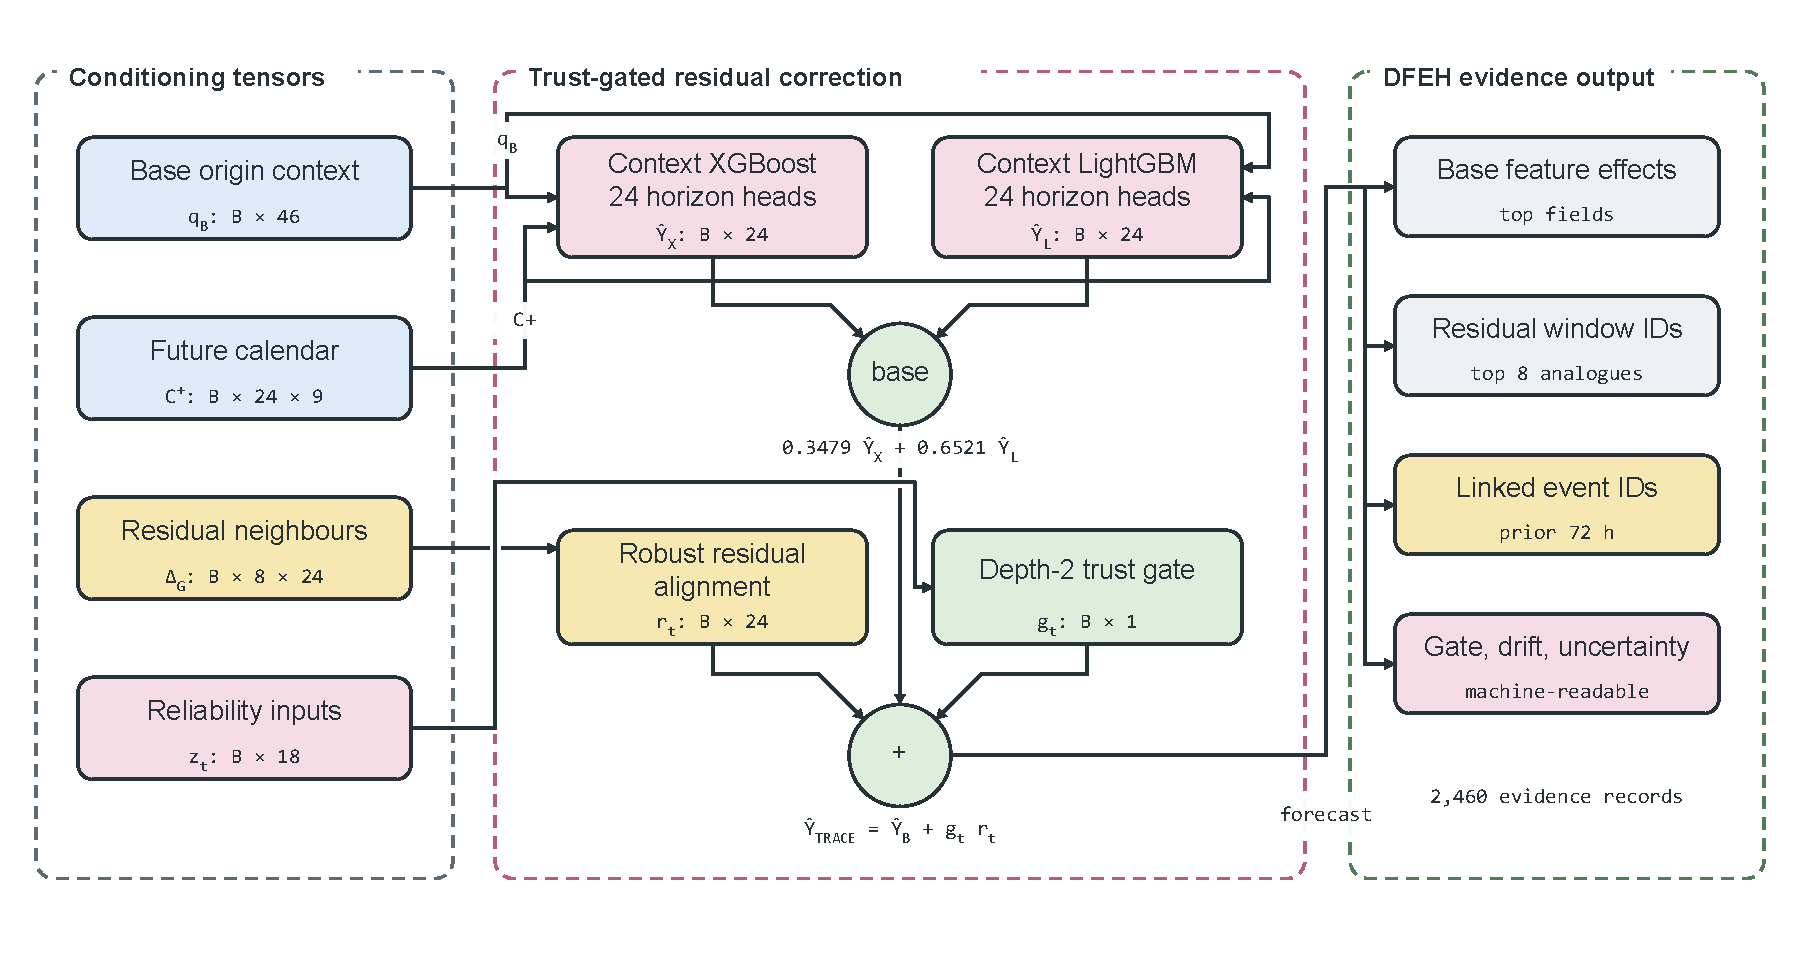
\includegraphics[width=\textwidth]{figures/drift_aware_forecast_evidence_head.pdf}
\caption{Drift-Aware Forecast and Evidence Head. Context, retrieval, drift, and
future-calendar tensors feed direct horizon regressors; the frozen
Chronos-Bolt path is fused only at forecast level. Stored feature effects,
retrieved cases, event identifiers, drift components, and uncertainty values
form the evidence record.}
\label{fig:explanation_flow}
\end{figure*}

\subsubsection{Feature-Level Forecasting and Drift Diagnostics}
Direct model input and prediction are for horizon $h$,
\begin{equation}
u_{t,h}=[q_t\,\|\,\rho(G_t)\,\|\,d_t\,\|\,c_{t+h}],
\qquad \hat{y}^{X}_{t+h}=f_h(u_{t,h}),
\label{eq:direct_heads}
\end{equation}
where $u_{t,h}\in\mathbb{R}^{151}$ for the entire M09 model, and each $f_h$ is an XGBoost regressor trained using a squared-error objective. This design allows for an independent supervised function per forecast horizon, but uses the same origin representation. Equation~(\ref{eq:direct_heads}) accounts for the 151 verified features: 85 context, 51 retrieval, six drift and nine future-calendar values. The drift score and binary flag are used for regime analysis and the evidence record, but not to adaptively pick a forecaster in the experiment reported.

\subsubsection{Frozen-TSFM Forecast Fusion}
The ``retrieval'' version of Chronos-Bolt is based on forecast-level fusion, not internal Channel Prompting. Let $\hat{Y}^{C}_t$ be the frozen Chronos forecast and $\hat{Y}^{R}_t$ be the retrieved historical forecast. The combination of forecasts is
\begin{equation}
    \hat{Y}^{CR}_t(\omega) =
    \omega \hat{Y}^{C}_t + (1-\omega)\hat{Y}^{R}_t,
    \label{eq:chronos_fusion}
\end{equation}
where $\omega\in\{0,0.25,0.5,0.75,1.0\}$ is selected on the validation split. Validation selected $\omega=0.75$. This branch does not modify Chronos-Bolt embeddings or weights as this takes place after both forecasts are made. Thus, the process given by the equation~(\ref{eq:chronos_fusion}) is an output space interpolation process, rather than an internal TSFM prompting operation.

\subsubsection{Concept-Drift Evidence}
The implementation represents distribution shift using transparent indicators; no claim is made toward perfect concept-drift identification. These indicators are recent mean shift, recent variance shift, retrieval similarity drop, weather-pattern shift and event-burst ratio. The raw vector used by the code is
\begin{equation}
\begin{aligned}
r_t=\bigg[&|\mu_{24,t}-\mu_{168,t}|,
\left|\log\frac{\sigma_{24,t}+\epsilon}{\sigma_{168,t}+\epsilon}\right|,
1-\operatorname{clip}(\bar{s}_{ts,t},0,1),\\
&\sqrt{\frac{1}{4}\sum_{\ell=1}^{4}
\left(\frac{w_{t,\ell}-\widetilde{w}^{tr}_{\ell}}
{s^{tr}_{w,\ell}}\right)^2},\ \max(b_{event,t},0)\bigg],
\end{aligned}
\label{eq:drift_raw}
\end{equation}
where the weather term is based on temperature, relative humidity, pressure and wind speed that have been standardized by training medians and standard deviations. The median and median absolute deviation (MAD) of the training data are then used to robustly scale each component $r_{t,j}$:
\begin{equation}
d_{t,j}=\frac{1}{6}\operatorname{clip}\left(
\frac{r_{t,j}-\operatorname{med}_{tr}(r_j)}
{\max(1.4826\operatorname{MAD}_{tr}(r_j),\epsilon)},0,6\right).
\label{eq:drift_scale}
\end{equation}
Lastly, the continuous score and binary flag are
\begin{equation}
S_t=\frac{1}{5}\sum_{j=1}^{5}d_{t,j},\qquad
D_t=\mathbb{I}\!\left[S_t\geq
Q_{0.90}\!\left(\{S_v:v\in\mathcal{T}_{val}\}\right)\right].
\label{eq:drift_score}
\end{equation}
Equations~(\ref{eq:drift_raw})--(\ref{eq:drift_score}) agree with the implemented detector: training data determine the reference statistics, validation data determine the 0.90-quantile threshold and test data are transformed without refitting. The binary $D_t$ is retained for diagnostic regime analysis and explanation evidence.

\subsubsection{Evidence Record and Diagnostic Scale}
The explanation module leverages signed local XGBoost contributions averaged across the 24 direct models, weather flags, top three retrieved windows, recent event records, calendar context, forecast direction, and component-level drift evidence. The local values are XGBoost TreeSHAP contributions returned by \texttt{pred\_contribs=True} after the bias column is removed, and then averaged across horizons. The diagnostic uncertainty scale is
\begin{equation}
u_t^{\mathrm{diag}}=
\sqrt{\bar{\sigma}_{R,t}^{2}+\overline{\mathrm{RMSE}}_{val}^{2}},
\label{eq:uncertainty_proxy}
\end{equation}
Here, $\bar{\sigma}_{R,t}$ is the mean horizon-wise spread of the retrieved trajectories while mean validation RMSE is the mean of the 24 horizon-wise validation RMSE values. The outcome is a diagnostic scale, rather than a calibrated prediction interval. Each explanation is constructed from fields stored in the system rather than from an unrestricted language model, and each event statement remains contextual rather than causal. Equation~(\ref{eq:uncertainty_proxy}) is retained only as an evidence-field definition and is not used to build confidence intervals.

\subsection{Relationship to TimeRAF}
TimeRAF extracts the top-k time-series windows by a learned MLP dual encoder and then merges the embedding of the candidate into a pre-trained TSFM via Channel Prompting \cite{zhang2025timeraf}. Table~\ref{tab:timeraf_comparison} lists the principles that are carried over and the mechanisms that are different. The comparison is methodological and not a performance ranking as different data sets, time horizons, and protocols have been used.

\begin{table*}[!t]
\centering
\caption{Methodological Comparison of TimeRAF and Event-TimeRAF}
\label{tab:timeraf_comparison}
\begin{tabular}{p{0.15\textwidth}p{0.38\textwidth}p{0.39\textwidth}}
\toprule
Aspect & TimeRAF & Event-TimeRAF \\
\midrule
Primary objective & Improve zero-shot forecasting by augmenting a frozen TSFM
with external time-series knowledge. & Evaluate source-audited, event-context
retrieval for local PM2.5 forecasting under temporal shift. \\
Forecasting domain & Multi-domain benchmark datasets. & Los Angeles County
hourly PM2.5, 2019--2024. \\
Knowledge base & Curated, consistently normalized time-series windows. & 1,521
training-history windows at the primary 24-hour stride, with denser and sparser
sensitivity settings, PM2.5, weather, calendar, and retrospective event context. \\
Retriever & Learned MLP dual encoder with forecaster-guided training. & Random,
cosine, and transparent hybrid similarity; no learned retriever. \\
Knowledge integration & Internal Channel Prompting of candidate embeddings. &
Feature-level XGBoost inputs and forecast-level Chronos-Bolt fusion. \\
Backbone & Frozen TSFM, principally TTM-Base. & Direct XGBoost horizon models
and frozen \texttt{amazon/chronos-bolt-small}. \\
Leakage control & Non-overlapping knowledge windows and cross-dataset training
constraints. & Candidate windows may overlap one another, but every candidate
target must end before the query lookback; validation and test use training
history only. \\
Event handling & Not an explicit module. & Availability-tagged NOAA Storm
Events features and source-record evidence, reported retrospectively. \\
Drift and explanation & Retrieved-case inspection. & Five-component drift
audit, signed feature effects, retrieved IDs, event IDs, and diagnostic scale. \\
Implementation scope & Learned retriever and Channel Prompting are implemented.
& Those mechanisms are not implemented and remain future extensions. \\
\bottomrule
\end{tabular}
\end{table*}
\section{Experimental Setup}

The final experiment is described in this section. Test evaluation was performed after model-selection choices were made using the training and validation partitions. Run identifier \texttt{20260810T103436161252Z} was used to check artifact consistency.

\subsection{Dataset Description and Audit}
The study period is 2019--2024. PM2.5 observations were obtained for Los Angeles County from US EPA AirData/AQS parameter 88101 \cite{epaairdata2026}. The official Los Angeles County AQS monitors were audited to obtain the hourly county median; no single monitor was targeted as the series. This fallback selected \texttt{06-037-COUNTY}, with 52,602 observed target hours and observed PM2.5 coverage of 0.9997. The PM2.5 unit is $\mu$g/m$^3$ per cubic meter ($\mu$g/m$^3$).

All weather covariates were obtained from NOAA Global Hourly/ISD, via NOAA Open Data Dissemination public buckets \cite{noaaisd2026}. This selected station was \texttt{72297023129} (Long Beach / Daugherty Field / Airport), 10.28 km from the PM2.5 target centroid. The total weather feature coverage (including past-only short gap filling) was 0.9942 and the raw measured coverage of the core weather variables was 0.9905.

Annual detail archives of NOAA Storm Events were loaded as environmental events, and the data were hash verified \cite{noaastormevents2026}. Due to the lack of direct access to NCEI in the execution environment, the experiment relied on a locally staged cache of unchanged NOAA annual archives and a source manifest file containing the official URLs, byte counts, and SHA-256 hashes of each archive. The delivery mode \texttt{verified\_official\_noaa\_cache} was retained in the audit. During the event audit, 117 event days and 2,192 source-overlap days were identified, as well as three qualifying event categories. High wind (76 records), flood (61) and other weather (40) meet the configured category threshold of 20 records; heavy rain (18) and wildfire (9) are retained but do not qualify. Event-aware outputs assume the recorded event start time as the retrospective availability time because NOAA Storm Events has no machine-readable publication timestamp. They are not strict real-time event forecasts. The resulting readiness status is given in Table~\ref{tab:data_audit}. Figure~\ref{fig:context_builder} shows the source audit window and window contract.

\begin{table}[!t]
\centering
\caption{Data-Readiness Audit}
\label{tab:data_audit}
\small
\setlength{\tabcolsep}{3pt}
\begin{tabular}{lccc}
\toprule
Gate & Observed & Requirement & Status \\
\midrule
PM2.5 coverage & 0.9997 & $\geq 0.70$ & Pass \\
Weather coverage & 0.9942 & $\geq 0.95$ & Pass \\
Event days & 117 & $\geq 30$ & Pass \\
Source-overlap days & 2,192 & $\geq 180$ & Pass \\
Qualifying categories & 3 & $\geq 2$ & Pass \\
Strict availability & False & --- & Caveat \\
\bottomrule
\end{tabular}
\end{table}

Window construction started from 52,608 aligned hourly rows and 52,417 possible forecast origins. It excluded 48 origins at split boundaries, eight for a missing lookback, 144 for a missing target and 3,885 for missing origin features, but none for future-calendar values. The remaining 48,332 origins comprise 34,020 training, 7,113 validation and 7,199 test origins.

\begin{table*}[!t]
\centering
\caption{Dataset and Source Summary}
\label{tab:dataset_summary}
\begin{tabular}{p{0.18\linewidth}p{0.27\linewidth}p{0.18\linewidth}p{0.25\linewidth}}
\toprule
Data group & Source & Evaluated scope & Use in pipeline \\
\midrule
PM2.5 & EPA AirData/AQS hourly parameter 88101 & Los Angeles County,
2019--2024; 52,602 observed target hours & Target sequence and lag/rolling
features \\
Weather & NOAA Global Hourly/ISD, station \texttt{72297023129} & 2019--2024;
0.9942 usable core coverage & Temperature, humidity, wind, pressure, and rain
features \\
Events & NOAA Storm Events annual detail archives & 204 Los Angeles records;
117 event days & Retrospective event-start features and explanation evidence \\
Calendar & Generated from timestamps and public holiday rules & 2019--2024
hourly calendar & Hour, weekday, weekend, month, season, and holiday features \\
\bottomrule
\end{tabular}
\end{table*}

Table~\ref{tab:dataset_summary} summarizes the scope evaluated, and the contribution of each source to the forecasting pipeline.

\subsection{Data and Code Availability}
EPA AirData \cite{epaairdata2026}, NOAA Global Hourly/ISD \cite{noaaisd2026} and NOAA Storm Events \cite{noaastormevents2026} provide access to the raw public records and download pages. In the execution environment there was no direct access to NCEI and the experiment employed a locally staged NOAA Storm Events cache, where every cached NOAA file was checked against the manifest that was generated during the experiment. The code can be found at \url{https://github.com/shasabbir/event-time-raf}. The implementation is based on Python 3.12.13, NumPy, pandas, scikit-learn, XGBoost, PyTorch and the \texttt{chronos-forecasting} package; all configuration, notebooks, source modules and tests are provided in the repository to reproduce the pipeline when the public sources are available.

\subsection{Forecasting Task and Split}
The forecasting task predicts PM2.5 for the next 1 to 24 hours with a lookback window of 168 hours. The split is chronological: the first 70\% of valid windows are used for training, the next 15\% for validation and the last 15\% for testing. The final test set has 7,199 forecast origins and 172,776 forecasted hourly target points. Test origins range from 7 February to 30 December 2024 UTC, while the test targets extend to 31 December 2024 UTC. Random splitting is not used.

\subsection{Models}
The models evaluated are persistence, daily seasonal naive, weekly seasonal naive, hourly-by-month climatology, ridge regression, direct XGBoost models, random, cosine, calendar-only and event-stratified retrieval, Event-TimeRAF without and with drift features, frozen Chronos-Bolt, and three Chronos fusion variants optimized using validation. The fusion controls replace retrieval with climatology or persistence while maintaining the weight-selection procedure. Ablation analysis uses an auxiliary random-retrieval XGBoost model (A01) and an event-free model (A00). A01 substitutes cosine retrieval features with seeded random retrieval features but keeps the context regressor. A00 omits event features and uses a four-component drift diagnostic and event-free hybrid retrieval. The \texttt{amazon/chronos-bolt-small} checkpoint is used for the foundation-model evaluation. Table~\ref{tab:model_families} classifies the assessed configurations by their forecasting and retrieval functions.

\begin{table}[!t]
\centering
\caption{Evaluated Model Families}
\label{tab:model_families}
\begin{tabular}{ll}
\toprule
ID & Description \\
\midrule
M00--M02 & Persistence and seasonal naive baselines \\
M03--M04 & XGBoost PM2.5-only and context models \\
M05--M06 & Random and cosine retrieval-only baselines \\
M07 & XGBoost with cosine retrieval features \\
M08--M09 & Event-TimeRAF without/with drift indicators \\
M10--M11 & Frozen Chronos-Bolt and retrieval fusion \\
C00--C03 & Climatology, ridge, calendar, and event-stratified controls \\
C10--C11 & Chronos climatology and persistence fusion controls \\
\bottomrule
\end{tabular}
\end{table}

\subsection{Implementation and Hyperparameters}
This experiment was performed in a cloud environment with Linux 6.12.90 and Python 3.12.13. The runtime was 3,319.95 seconds. Package versions included in the run manifest are NumPy 2.0.2, pandas 2.3.3, scikit-learn 1.6.1, XGBoost 3.2.0, PyTorch 2.10.0+cu128 and \texttt{chronos-forecasting} 2.3.1. The main hyperparameters are given in Table~\ref{tab:hyperparameters}.

\begin{table*}[!t]
\centering
\caption{Experimental Hyperparameters and Runtime Settings}
\label{tab:hyperparameters}
\renewcommand{\arraystretch}{0.94}
\begin{tabular}{ll}
\toprule
Component & Setting \\
\midrule
Study period & 2019--2024 \\
Lookback and horizon & $L=168$ hours, $H=24$ hours \\
Split & 70\% train, 15\% validation, 15\% test, chronological \\
SACB feature groups & 23 PM2.5, 14 weather, 9 calendar, 39 event features \\
SACB missing-data rule & Past-only filling for gaps up to 3 hours; no target interpolation \\
LSER retrieval & $k=8$, sensitivity for $k \in \{1,4,8,16\}$ \\
LSER knowledge base & 1,521 windows at 24-hour primary stride; sensitivity at 192, 24, 6, and 1 hours \\
LSER similarity weights & time series 0.5, weather 0.2, calendar 0.1, event 0.2 \\
LSER event-weight sensitivity & $\delta\in\{0,0.2,0.5,0.8,1.0\}$ with remaining weights renormalized \\
DFEH direct input & 151 features for each of 24 horizon regressors \\
DFEH XGBoost & 350 estimators, max depth 6, learning rate 0.05, subsample 0.85,
colsample 0.85, $\lambda=1.0$ \\
DFEH drift detector & 5 components; 24-hour recent window, 168-hour reference window,
0.90 validation quantile threshold \\
DFEH Chronos path & \texttt{amazon/chronos-bolt-small}, batch size 64 \\
DFEH fusion weights & $\{0,0.25,0.5,0.75,1.0\}$; selected $\omega=0.75$ \\
Explanation record & Top 3 feature effects, windows, and recent event IDs \\
Inference & 2,000 paired block-bootstrap resamples, 168-origin blocks; DM HAC lag 167; Holm adjustment \\
\bottomrule
\end{tabular}
\end{table*}

\subsection{Evaluation Metrics and Statistical Checks}
The metrics of interest are MSE, MAE, RMSE, MAPE, sMAPE, and $R^2$. MSE is kept for comparison to the TimeRAF evaluation, and MAE and RMSE offer more comprehensible PM2.5 error scales. The main error measures are, for the $n$ observed forecast values $y_j$ and the predictions $\hat{y}_j$:
\begin{equation}
\begin{aligned}
\operatorname{MSE}&=\frac{1}{n}\sum_{j=1}^{n}(y_j-\hat{y}_j)^2,\\
\operatorname{MAE}&=\frac{1}{n}\sum_{j=1}^{n}|y_j-\hat{y}_j|,\\
\operatorname{RMSE}&=\sqrt{\operatorname{MSE}},
\end{aligned}
\label{eq:error_metrics}
\end{equation}
Explained variance is summarized by Equation~(\ref{eq:r2_metric}).
\begin{equation}
R^2=1-\frac{\sum_{j=1}^{n}(y_j-\hat{y}_j)^2}
{\sum_{j=1}^{n}(y_j-\bar{y})^2}.
\label{eq:r2_metric}
\end{equation}
The overall result is obtained by aggregating across all the forecast origins and horizons as given in Equation~(\ref{eq:error_metrics}) and the same set of points is used in (\ref{eq:r2_metric}). However, due to the uncertainty of percentage errors when PM2.5 levels are low, MAPE and sMAPE are reported in machine-readable outputs, but not used to rank the results. Subset metrics are only reported if there are 50 or more forecast origins. All pre-specified subsets meet the minimum sample-size criterion and they number 532 origins in the event subset, 293 in the active-event subset and 566 in the drift subset. The primary pairwise comparisons are based on 2,000 paired block-bootstrap resamples with 168-origin blocks. Diebold--Mariano tests are performed with a Newey--West/HAC variance estimate with lag 167, and Holm adjustment for each pre-specified metric family.

\subsection{Comparison with Existing Studies}
The direct comparison of the numerical results with previous studies on TSFM and air quality is not possible due to the use of different datasets, forecast horizons, variables and evaluation protocol. It must therefore be noted that Table~\ref{tab:literature_positioning} is a comparison of methodological coverage and not a cross-paper comparison of performance.

\begin{table*}[!t]
\centering
\caption{Methodological Comparison with Related Forecasting Work}
\label{tab:literature_positioning}
\begin{tabular}{p{0.18\linewidth}ccccp{0.27\linewidth}}
\toprule
Method family & TSFM & Retrieval & Events & Explainability & Comment \\
\midrule
PatchTST-style Transformers \cite{nie2023patchtst} & No & No & No & Limited &
Strong sequence modeling, but event context is not central. \\
Chronos \cite{ansari2024chronos} & Yes & No & No & Limited & Frozen
zero-shot baseline used in this study. \\
TimeRAF \cite{zhang2025timeraf} & Yes & Yes & No & Retrieval cases & Base
retrieval-augmented TSFM method; does not target official event-aware PM2.5. \\
XGBoost context baseline \cite{chen2016xgboost} & No & No & No & Feature
importance & Strong supervised tabular baseline for local PM2.5. \\
Event-TimeRAF & Yes & Yes & Yes & Evidence-grounded & Adds official event
audit, temporal leakage control, drift indicators, and Chronos retrieval fusion. \\
\bottomrule
\end{tabular}
\end{table*}
\section{Results and Discussion}

\subsection{Overall Comparison with Baselines}
The results of the test set are shown in Table~\ref{tab:main_results}. M04, which is based on PM2.5 history, weather and calendar features, is the best pre-specified supervised model with MSE 26.185, MAE 3.125, RMSE 5.117 and $R^2$ 0.379. The complete feature-level Event-TimeRAF model M09 achieves the following scores: MSE 26.734 and MAE 3.144. So, the full event, retrieval and drift feature set does not improve the all-origin error compared to the simpler context model.

\begin{table*}[!t]
\centering
\caption{Manifest-Backed Overall Test Results for 24-Hour PM2.5 Forecasting}
\label{tab:main_results}
\begin{tabular}{lrrrr}
\toprule
Model & MSE & MAE & RMSE & $R^2$ \\
\midrule
C00 hour--month climatology & 36.297 & 4.038 & 6.025 & 0.139 \\
C01 ridge context & 28.448 & 3.226 & 5.334 & 0.325 \\
C02 calendar retrieval & 45.534 & 4.429 & 6.748 & -0.080 \\
C03 event-stratified retrieval & 38.428 & 3.924 & 6.199 & 0.089 \\
M00 persistence & 47.649 & 4.137 & 6.903 & -0.130 \\
M01 daily seasonal & 48.706 & 4.057 & 6.979 & -0.155 \\
M02 weekly seasonal & 65.606 & 5.123 & 8.100 & -0.556 \\
M03 XGBoost PM2.5 & 29.949 & 3.368 & 5.473 & 0.290 \\
M04 XGBoost context & \textbf{26.185} & \textbf{3.125} & \textbf{5.117} & \textbf{0.379} \\
M05 random retrieval & 44.089 & 4.346 & 6.640 & -0.046 \\
M06 cosine retrieval & 36.243 & 3.818 & 6.020 & 0.140 \\
M07 XGBoost cosine & 26.442 & 3.132 & 5.142 & 0.373 \\
M08 Event-TimeRAF no drift & 26.700 & 3.144 & 5.167 & 0.367 \\
M09 Event-TimeRAF full & 26.734 & 3.144 & 5.171 & 0.366 \\
M10 frozen Chronos-Bolt & 28.941 & 3.205 & 5.380 & 0.314 \\
M11 Chronos + retrieval & 28.733 & 3.205 & 5.360 & 0.319 \\
C10 Chronos + climatology & 27.450 & 3.137 & 5.239 & 0.349 \\
C11 Chronos + persistence & 28.941 & 3.205 & 5.380 & 0.314 \\
\bottomrule
\end{tabular}
\end{table*}

The frozen Chronos-Bolt evaluation completed successfully. A retrieval-fusion weight of 0.75 was selected through validation. On the test set, M11 changes MSE from 28.941 to 28.733. The M11--M10 difference is -0.209 with a 95\% block-bootstrap interval $[-0.654,0.216]$ and Holm-adjusted DM $p=1.000$, so the change is unresolved. The matched climatology fusion C10 obtains MSE 27.450. M11 is worse than C10 by 1.283 MSE, with interval $[0.694,1.913]$ and adjusted $p<0.001$. The persistence control selects a TSFM weight of 1.0 and therefore equals M10. This experiment thus does not identify a retrieval-specific advantage: ordinary validation-tuned forecast combination performs better.

\subsection{Ablation Study}
Comparisons on a component basis are summarized in Table~\ref{tab:ablation_results}. The MSE is reduced by 3.764 using weather and calendar context over PM2.5-only XGBoost, and cosine retrieval improves substantially over random retrieval when retrieval only is used. All the other feature-level additions contain intervals that cross zero. Specifically, M09 is 0.550 MSE worse than M04, and its difference from event-free A00 is unresolved. Drift indicators change M08 by only 0.034 MSE. These results do not support a monotone accuracy contribution from each named module.

\begin{table*}[!t]
\centering
\caption{Selected Paired Block-Bootstrap Ablation Results}
\label{tab:ablation_results}
\begin{tabular}{lrrrr}
\toprule
Comparison & MSE diff. & 95\% CI low & 95\% CI high & Holm DM $p$ \\
\midrule
M04 minus M03, weather/calendar & -3.764 & -7.120 & -1.709 & 0.067 \\
M06 minus M05, cosine/random retrieval & -7.846 & -11.333 & -4.849 & --- \\
M07 minus M04, retrieval summary & 0.258 & -0.269 & 1.012 & --- \\
M08 minus M07, event-hybrid ranking & 0.258 & -0.087 & 0.690 & --- \\
M09 minus M08, drift indicators & 0.034 & -0.079 & 0.147 & --- \\
M09 minus A00, event context & 0.216 & -0.114 & 0.635 & 1.000 \\
M09 minus M04, complete feature path & 0.550 & -0.122 & 1.592 & 1.000 \\
M11 minus M10, retrieval fusion & -0.209 & -0.654 & 0.216 & 1.000 \\
M11 minus C10, climatology placebo & 1.283 & 0.694 & 1.913 & $<0.001$ \\
\bottomrule
\end{tabular}
\end{table*}

Intervals are paired block-bootstrap intervals. The pre-specified primary family is used to display the Holm adjusted DM values; dashes indicate secondary diagnostic comparisons, not missing experiment runs.

Table~\ref{tab:k_sensitivity} shows that the retrieval-only cosine baseline improves as the number of neighbours increases within the tested range. The best retrieval-only configuration among $k\in\{1,4,8,16\}$ is $k=16$, with MSE 34.440. All the reported Event-TimeRAF feature models were based on the pre-specified default $k=8$.

\begin{table}[!t]
\centering
\caption{Cosine Retrieval Sensitivity to $k$}
\label{tab:k_sensitivity}
\begin{tabular}{rrrr}
\toprule
$k$ & MSE & MAE & RMSE \\
\midrule
1 & 60.555 & 4.886 & 7.782 \\
4 & 40.004 & 4.010 & 6.325 \\
8 & 36.243 & 3.818 & 6.020 \\
16 & 34.440 & 3.711 & 5.869 \\
\bottomrule
\end{tabular}
\end{table}

\subsection{Knowledge-Base Density and Event Sensitivity}
Table~\ref{tab:stride_sensitivity} demonstrates that the original sparse-memory issue has implications for retrieval alone. Decreasing the stride from 192 to six hours increases the number of candidates from 191 to 5,644 and reduces retrieval-only MSE from 39.037 to 34.616. A one-hour stride is not better than the six-hour stride. The separately trained full feature model also gives its lowest observed MSE at six hours (26.412), but it remains behind M04 (26.185). Dense retrieval therefore enhances the historical analogue baseline without changing the overall model ranking.

\begin{table*}[!t]
\centering
\caption{Knowledge-Base Stride Sensitivity on the Test Set}
\label{tab:stride_sensitivity}
\begin{tabular}{rrrrr}
\toprule
Stride (h) & Candidates & Retrieval MSE & Retrieval MAE & Full M09 MSE \\
\midrule
192 & 191 & 39.037 & 3.991 & 26.712 \\
24 & 1,521 & 38.411 & 3.921 & 26.734 \\
6 & 5,644 & \textbf{34.616} & \textbf{3.660} & \textbf{26.412} \\
1 & 34,020 & 36.416 & 3.790 & 26.740 \\
\bottomrule
\end{tabular}
\end{table*}

The event channel is active but is not helpful under the tested representation. At weight 0.2 it changes at least one of the top-8 candidates for 91.4\% of test queries and increases the event-candidate fraction for event-context queries from 32.9\% to 95.7\%. However, Table~\ref{tab:event_weight_sensitivity} indicates that the all-origin and event-subset errors increase as the event weight rises. Event-stratified retrieval is also worse than the event-free ranking. The conclusion supported by this study is not that there is no forecast signal in environmental events, but rather that this count-based event representation and ranking rule is ineffective.

\begin{table*}[!t]
\centering
\caption{Event-Channel Sensitivity for Retrieval-Only Forecasts}
\label{tab:event_weight_sensitivity}
\begin{tabular}{lrrrr}
\toprule
Method & Event weight & Top-$k$ changed & All-origin MSE & Event-subset MSE \\
\midrule
Hybrid & 0.0 & 0.000 & \textbf{38.080} & \textbf{14.299} \\
Hybrid & 0.2 & 0.914 & 38.411 & 16.401 \\
Hybrid & 0.5 & 0.914 & 38.703 & 19.292 \\
Hybrid & 0.8 & 0.914 & 38.969 & 21.201 \\
Hybrid & 1.0 & 1.000 & 40.860 & 27.130 \\
Event-stratified & 0.2 & 0.917 & 38.428 & 16.638 \\
\bottomrule
\end{tabular}
\end{table*}

\subsection{Event and Drift Subsets}
Representative event and drift subsets for the strongest context model, the full Event-TimeRAF model and the two Chronos variants are reported in Table~\ref{tab:event_drift_results}. All subsets meet pre-specified minimum sample size. Variance of event targets is 22.636, variance of non-event targets is 43.346, variance of drift targets is 69.593 and variance of non-drift targets is 39.826. Raw subset MSE is consequently a measure of model error and target difficulty. The drift subset consists of all samples with the validation-calibrated DFEH flag, and is only employed for stratified evaluation.

\begin{table*}[!t]
\centering
\caption{Representative Event and Drift Subset Results}
\label{tab:event_drift_results}
\begin{tabular}{llrrr}
\toprule
Subset & Model & Origins & MSE & MAE \\
\midrule
Non-event & M04 XGBoost context & 6,667 & 27.520 & 3.179 \\
Event & M04 XGBoost context & 532 & 9.451 & 2.450 \\
Non-event & M09 Event-TimeRAF full & 6,667 & 27.995 & 3.187 \\
Event & M09 Event-TimeRAF full & 532 & 10.932 & 2.613 \\
Non-drift & M04 XGBoost context & 6,633 & 26.060 & 3.086 \\
Drift & M04 XGBoost context & 566 & 27.650 & 3.585 \\
Non-drift & M09 Event-TimeRAF full & 6,633 & 26.282 & 3.085 \\
Drift & M09 Event-TimeRAF full & 566 & 32.039 & 3.833 \\
Drift & M10 frozen Chronos-Bolt & 566 & 29.539 & 3.524 \\
Drift & M11 Chronos + retrieval & 566 & 29.210 & 3.610 \\
\bottomrule
\end{tabular}
\end{table*}

\subsection{Horizon-Wise and Retrieval Diagnostics}
Fig.~\ref{fig:mse_horizon} and Fig.~\ref{fig:mae_horizon} present test error by forecast horizon. Retrieval behaviour is summarized in Figure~\ref{fig:retrieval_diagnostics}, and the distribution of drift scores over the test period is presented in Figure~\ref{fig:drift_scores}. A representative test-origin forecast is shown in Figure~\ref{fig:forecast_case}, where M04 and M09 can be compared with the observed test target. These plots were recreated from predictions identified by run \texttt{20260810T103436161252Z}. The upper-tail drift threshold flags 712 of 7,113 validation origins (10.0\%) and 566 of 7,199 test origins (7.9\%). This difference is a diagnostic property; the flag does not change models or establish that concept drift occurred.

\begin{figure}[!t]
\centering

\includegraphics[width=0.95\columnwidth]{figures/mse_by_horizon.png}
\caption{MSE by forecast horizon on the Los Angeles County test set.}
\label{fig:mse_horizon}
\end{figure}

\begin{figure}[!t]
\centering
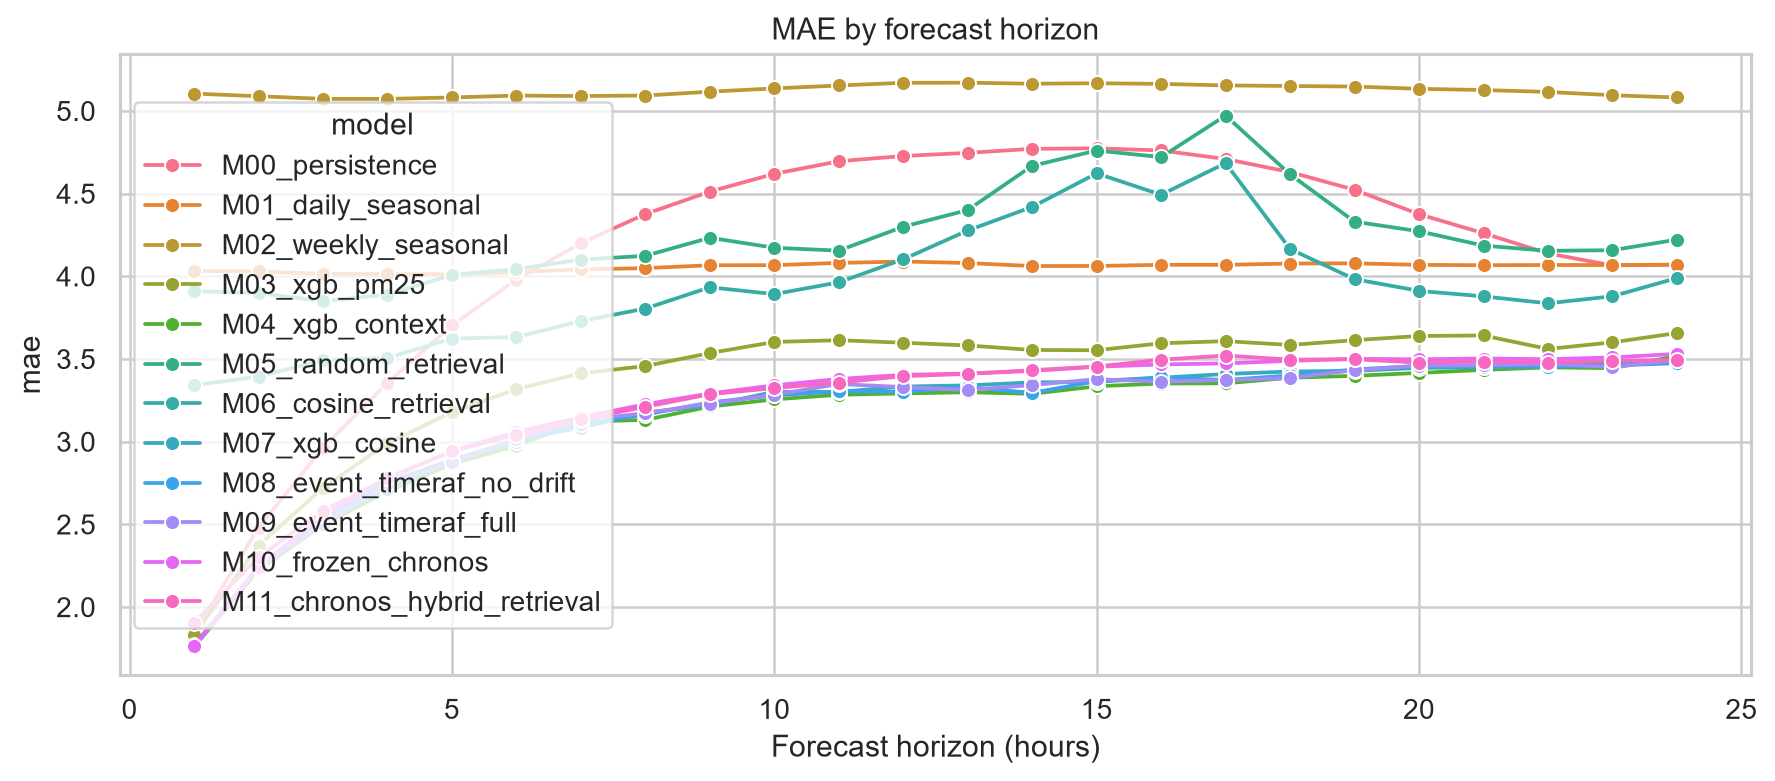
\includegraphics[width=0.95\columnwidth]{figures/mae_by_horizon.png}
\caption{MAE by forecast horizon on the Los Angeles County test set.}
\label{fig:mae_horizon}
\end{figure}

\begin{figure}[!t]
\centering
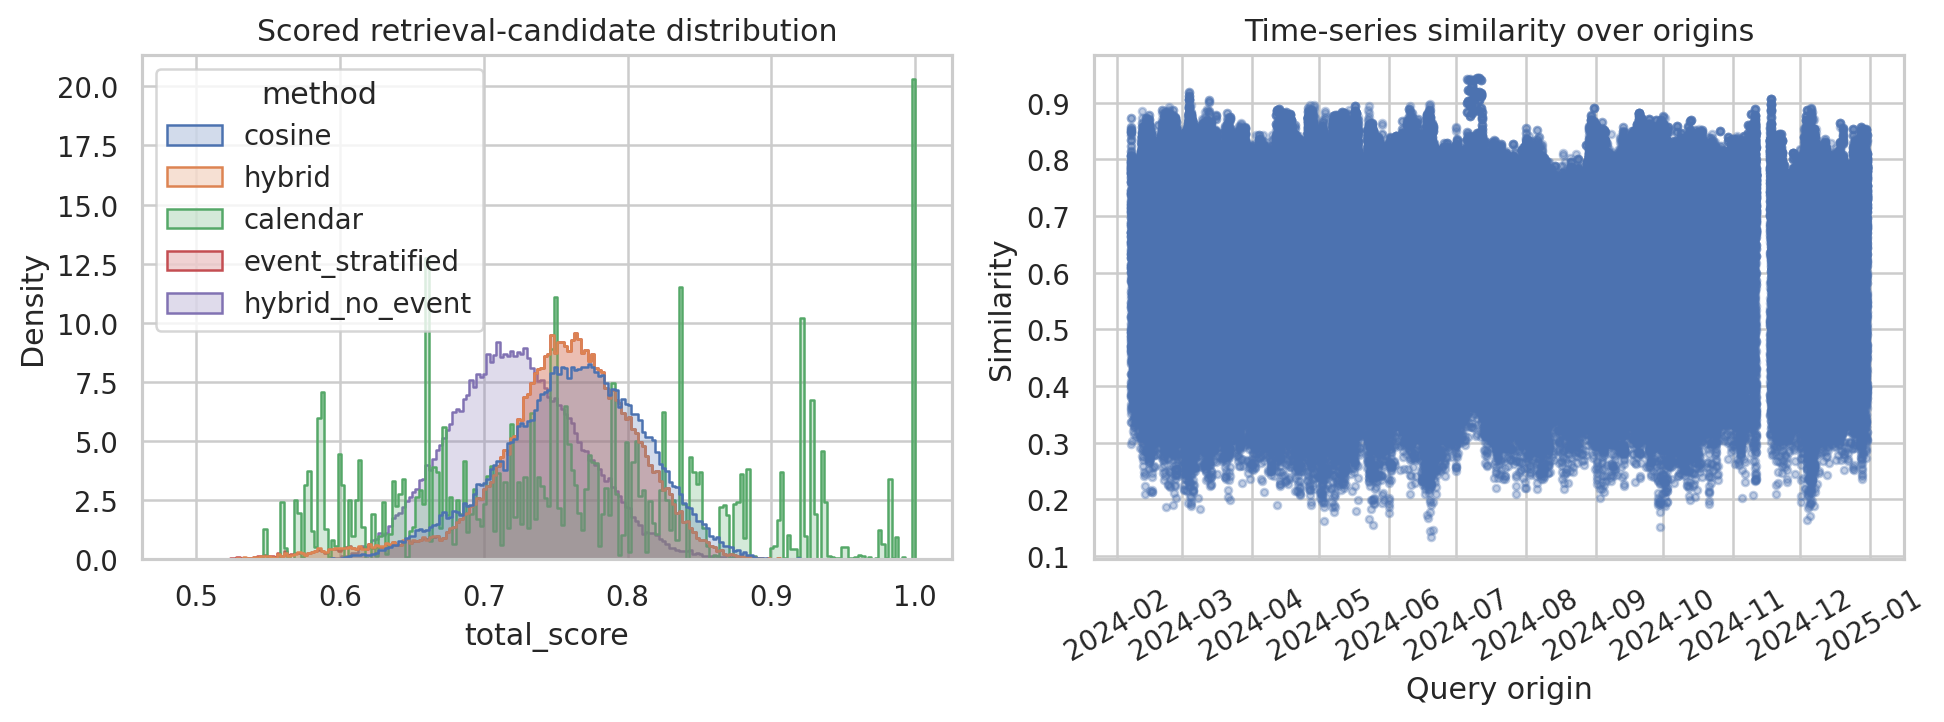
\includegraphics[width=0.95\columnwidth]{figures/retrieval_diagnostics.png}
\caption{Similarity and candidate diagnostics for test-set retrieval.}
\label{fig:retrieval_diagnostics}
\end{figure}

\begin{figure}[!t]
\centering
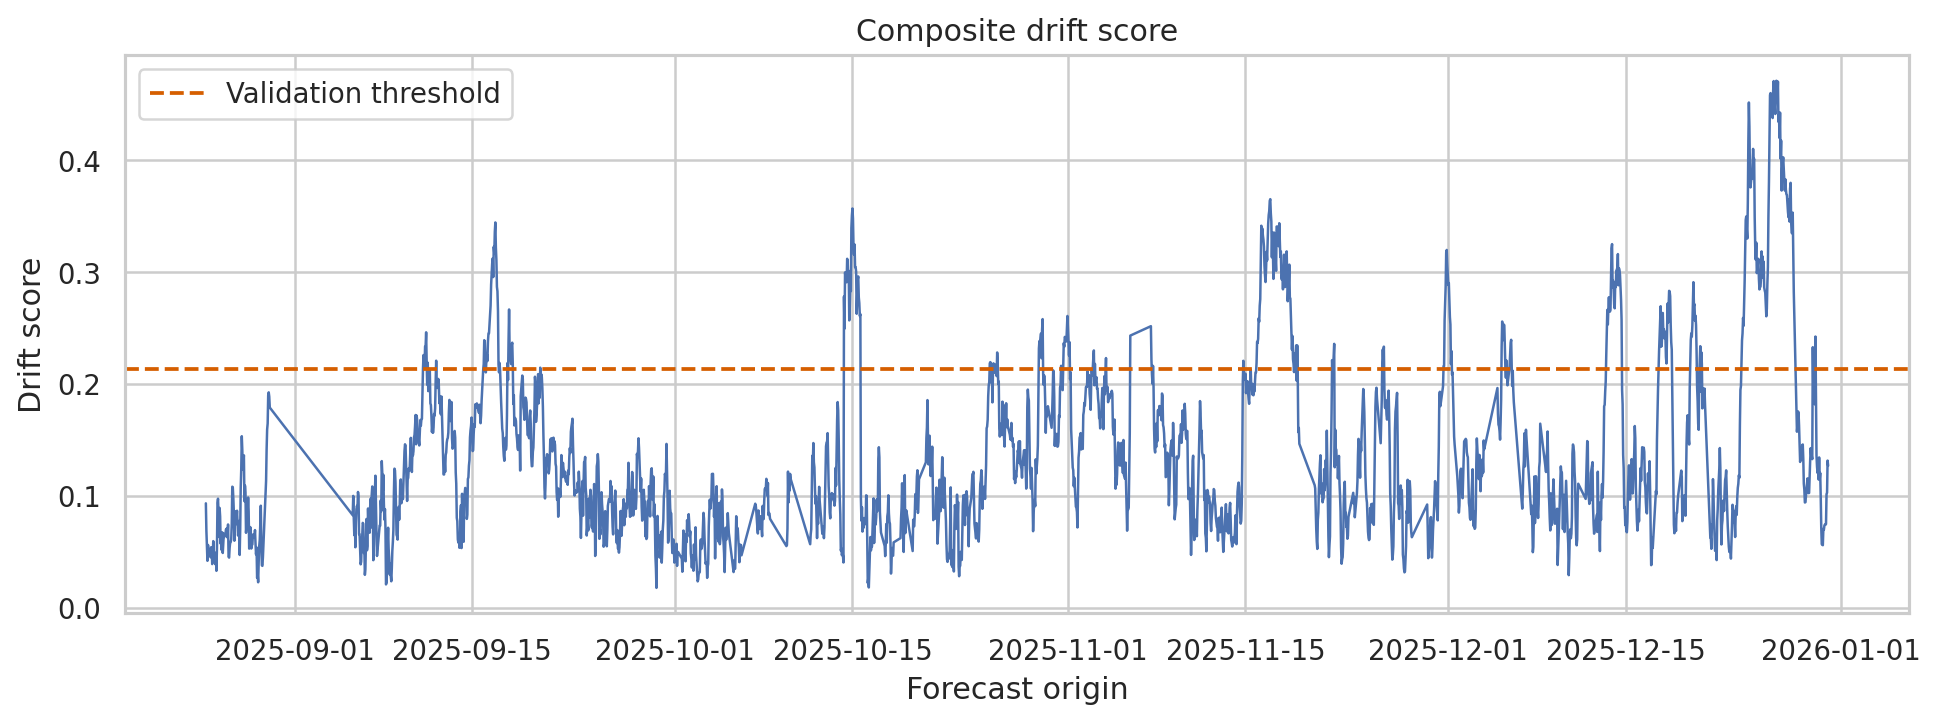
\includegraphics[width=0.95\columnwidth]{figures/drift_scores.png}
\caption{Composite drift-score diagnostics on the test set.}
\label{fig:drift_scores}
\end{figure}

\begin{figure}[!t]
\centering
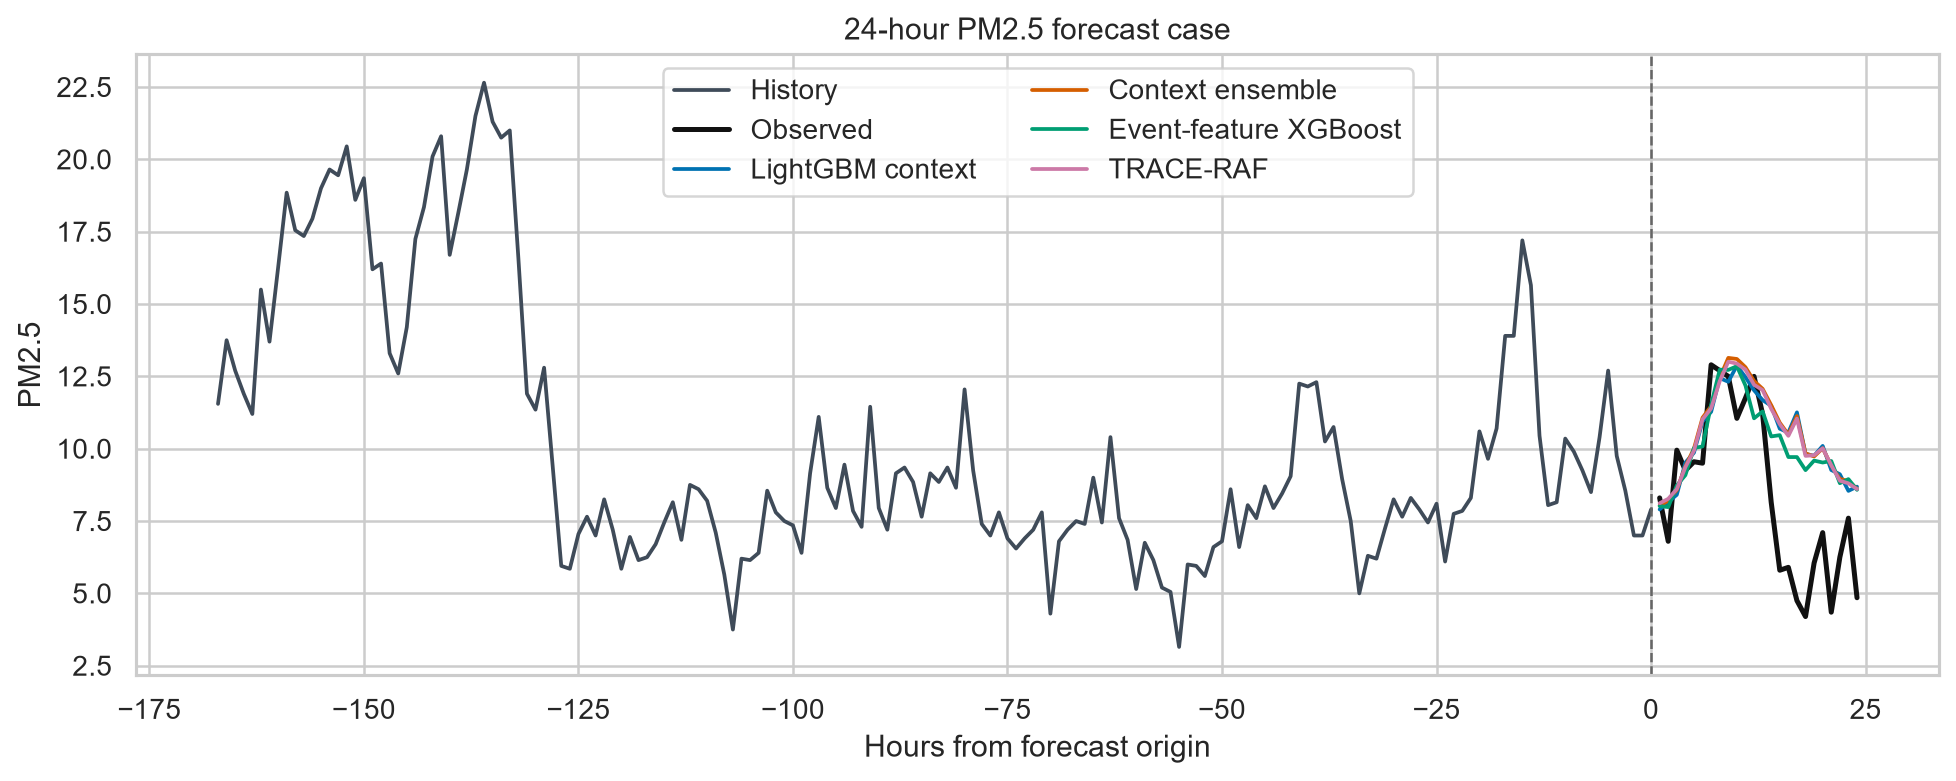
\includegraphics[width=0.95\columnwidth]{figures/forecast_case.png}
\caption{Representative 24-hour forecast case from the test set.}
\label{fig:forecast_case}
\end{figure}

\subsection{Evidence and Traceability Analysis}

In the DFEH, traceability is implemented as a source-embedded evidence record instead of a post-hoc, free-text interpretation. The run identifier, window identifier, origin timestamp, retrieved historical evidence identifiers, event evidence identifiers, leading feature effects, drift components, retrieval spread, validation residual RMSE, diagnostic uncertainty scale, drift score, drift flag and event-availability mode are stored for each evaluated forecast origin. The evaluation resulted in 7,199 explanation records in \texttt{explanations.parquet}. A representative record shows that the highest local contribution fields are the current PM2.5 value and recent rolling PM2.5 means, associates the prediction with three retrieved historical windows and recent source-recorded storm events when present, and marks distribution shift when the drift detector is active.

An explanation layer is summarized in Table~\ref{tab:explainability_outputs}. This design allows for auditability as every explanatory statement is linked to either a model feature or to a retrieved time-series window, official event record or drift component. It is not necessarily causal -- evidence of event is reported as contextual support and the drift flag is an uncertainty warning.

Chronos-Bolt's nominal 80\% interval has 78.2\% test-target coverage with a mean width of 9.890 $\mu$g/m$^3$. This interval result is distinct from the \texttt{diagnostic\_uncertainty\_scale} in the evidence record, which combines retrieval spread and validation residual RMSE and is not a calibrated interval.

\begin{table}[!t]
\centering
\caption{Explanation Evidence Stored by Event-TimeRAF}
\label{tab:explainability_outputs}
\begin{tabular}{p{0.33\columnwidth}p{0.57\columnwidth}}
\toprule
Evidence field & Interpretation role \\
\midrule
Top feature effects & Local model drivers from the direct forecaster. \\
Retrieved windows & Historical analogues used by the retrieval module. \\
Event evidence IDs & Official storm-event context linked to the origin. \\
Drift components & Mean, variance, weather, similarity, and event-burst shift signals. \\
Diagnostic scale & Combined retrieval spread and validation residual RMSE; not a calibrated interval. \\
\bottomrule
\end{tabular}
\end{table}

\subsection{Computational Cost and Reproducibility}

The entire experiment was run in 3,319.95 seconds in a cloud-hosted Linux environment using Python 3.12.13. The recorded package versions include NumPy 2.0.2, pandas 2.3.3, scikit-learn 1.6.1, XGBoost 3.2.0, PyTorch 2.10.0+cu128 and \texttt{chronos-forecasting} 2.3.1. The run manifest records the configuration SHA-256 hash and artifact checksums. The model identifiers for the CPU, GPU and RAM were not stored in the manifest; therefore, this paper reports only runtime and software versions and makes no claim about hardware-normalized efficiency. Table~\ref{tab:compute_summary} lists the reproducibility fields retained in the archived run.

\begin{table}[!t]
\centering
\caption{Computational and Reproducibility Summary}
\label{tab:compute_summary}
\begin{tabular}{ll}
\toprule
Item & Recorded value \\
\midrule
Run identifier & \texttt{20260810T103436161252Z} \\
Runtime & 3,319.95 seconds \\
Platform & Cloud-hosted Linux environment \\
Python & 3.12.13 \\
Forecast horizon & 24 hours \\
Lookback window & 168 hours \\
Bootstrap resamples & 2,000; block length 168 origins \\
Chronos checkpoint & \texttt{amazon/chronos-bolt-small} \\
Code availability & \url{https://github.com/shasabbir/event-time-raf} \\
\bottomrule
\end{tabular}
\end{table}

The predominant interpretation is that conventional context features are strong for this Los Angeles County task. The retrieval-only baseline is enhanced by dense historical memory, but retrieval, event and drift features do not outperform M04. The small M11 change relative to frozen Chronos remains unresolved, and the climatology fusion control significantly outperforms M11. Event-TimeRAF is thus evidence of a protocol for auditable evaluation and a scoped negative result, but not evidence for retrieval-specific or event-specific superiority.

Finally, all event-aware interpretations must be read with the availability caveat. NOAA Storm Events records are official and hash verified, but publication time is not provided in machine-readable format. For the experiment, the availability time is the event start time; therefore, event-related results are retrospective sensitivity results. A strict operational study would require event or smoke sources with genuine issue or publication times, such as an audited NOAA HMS cache or alert product archive.
\section{Limitations}

The first restriction concerns event availability. NOAA Storm Events records are official and hash verified, but the public detail files do not include machine-readable publication times. The SACB therefore uses event start as an availability proxy, making event-conditioned results retrospective sensitivity analyses rather than operational forecasts.

The second limitation is the geographic validation. The experiment spans an aggregate of PM2.5 for one county over the time period of 2019 to 2024. It does not claim transfer to another county, monitoring topology, climate or emissions regime, and thus is not a full-fledged generalization according to the external-validation criterion for a mature generalization claim.

The third constraint is related to model integration. The LSER is based on transparent similarity functions, and the DFEH combines Chronos-Bolt and retrieval only at forecast level. Thus, Event-TimeRAF does not duplicate TimeRAF's trained dual encoder or built-in Channel Prompting.

The fourth limitation is with respect to the reporting of computations. Runtime could not be interpreted as a hardware-normalized efficiency result as the run manifest was missing hardware model-identifiers and peak memory.

The fifth constraint is target aggregation. The hourly county median combines a changing group of monitors and suppresses local extremes. This enhances series continuity but may weaken event associations and prevents conclusions regarding individual neighborhoods or monitoring sites.

\section{Future Work}

Operational event studies should use archives that provide genuine issue or publication times and should consider sources more closely related to PM2.5, such as smoke observations, in place of event-start proxies. The same protocol should be applied to a second US county with different meteorology and emissions. Future research could test targets at the site level, a learned retriever for event context, more expressive event embeddings, calibrated probabilistic uncertainty, and conditioning in the TSFM. The source audit, temporal embargo and component-wise controls used here should be maintained in each extension.
\section{Conclusion}

This study audited event-aware retrieval for 24-hour PM2.5 forecasting in Los Angeles County. The pipeline synchronizes official environmental records, implements a query--candidate temporal embargo, checks memory density and event-channel sensitivity, and retains traceable evidence. M04 is the strongest evaluated model, with MSE 26.185, MAE 3.125, RMSE 5.117, and $R^2$ 0.379; full M09 obtains MSE 26.734. M11 changes frozen Chronos-Bolt MSE from 28.941 to 28.733, but the paired interval crosses zero, while climatology fusion reaches 27.450 and significantly outperforms M11. Dense retrieval improves the retrieval-only path, whereas the tested event channel does not improve it. The contribution is therefore a reproducible evaluation and a bounded negative finding: historical retrieval can be implemented under a verified query--candidate temporal embargo and audited extensively without necessarily providing forecast value beyond strong local context and straightforward forecast combination.

\bibliographystyle{IEEEtran}
\bibliography{references}

\end{document}
